% Options for packages loaded elsewhere
\PassOptionsToPackage{unicode}{hyperref}
\PassOptionsToPackage{hyphens}{url}
\PassOptionsToPackage{dvipsnames,svgnames,x11names}{xcolor}
%
\documentclass[
  12pt,
  letterpaper,
]{book}

\usepackage{amsmath,amssymb}
\usepackage{iftex}
\ifPDFTeX
  \usepackage[T1]{fontenc}
  \usepackage[utf8]{inputenc}
  \usepackage{textcomp} % provide euro and other symbols
\else % if luatex or xetex
  \usepackage{unicode-math}
  \defaultfontfeatures{Scale=MatchLowercase}
  \defaultfontfeatures[\rmfamily]{Ligatures=TeX,Scale=1}
\fi
\usepackage{lmodern}
\ifPDFTeX\else  
    % xetex/luatex font selection
\fi
% Use upquote if available, for straight quotes in verbatim environments
\IfFileExists{upquote.sty}{\usepackage{upquote}}{}
\IfFileExists{microtype.sty}{% use microtype if available
  \usepackage[]{microtype}
  \UseMicrotypeSet[protrusion]{basicmath} % disable protrusion for tt fonts
}{}
\makeatletter
\@ifundefined{KOMAClassName}{% if non-KOMA class
  \IfFileExists{parskip.sty}{%
    \usepackage{parskip}
  }{% else
    \setlength{\parindent}{0pt}
    \setlength{\parskip}{6pt plus 2pt minus 1pt}}
}{% if KOMA class
  \KOMAoptions{parskip=half}}
\makeatother
\usepackage{xcolor}
\usepackage[margin=1in]{geometry}
\setlength{\emergencystretch}{3em} % prevent overfull lines
\setcounter{secnumdepth}{5}
% Make \paragraph and \subparagraph free-standing
\makeatletter
\ifx\paragraph\undefined\else
  \let\oldparagraph\paragraph
  \renewcommand{\paragraph}{
    \@ifstar
      \xxxParagraphStar
      \xxxParagraphNoStar
  }
  \newcommand{\xxxParagraphStar}[1]{\oldparagraph*{#1}\mbox{}}
  \newcommand{\xxxParagraphNoStar}[1]{\oldparagraph{#1}\mbox{}}
\fi
\ifx\subparagraph\undefined\else
  \let\oldsubparagraph\subparagraph
  \renewcommand{\subparagraph}{
    \@ifstar
      \xxxSubParagraphStar
      \xxxSubParagraphNoStar
  }
  \newcommand{\xxxSubParagraphStar}[1]{\oldsubparagraph*{#1}\mbox{}}
  \newcommand{\xxxSubParagraphNoStar}[1]{\oldsubparagraph{#1}\mbox{}}
\fi
\makeatother

\usepackage{color}
\usepackage{fancyvrb}
\newcommand{\VerbBar}{|}
\newcommand{\VERB}{\Verb[commandchars=\\\{\}]}
\DefineVerbatimEnvironment{Highlighting}{Verbatim}{commandchars=\\\{\}}
% Add ',fontsize=\small' for more characters per line
\usepackage{framed}
\definecolor{shadecolor}{RGB}{241,243,245}
\newenvironment{Shaded}{\begin{snugshade}}{\end{snugshade}}
\newcommand{\AlertTok}[1]{\textcolor[rgb]{0.68,0.00,0.00}{#1}}
\newcommand{\AnnotationTok}[1]{\textcolor[rgb]{0.37,0.37,0.37}{#1}}
\newcommand{\AttributeTok}[1]{\textcolor[rgb]{0.40,0.45,0.13}{#1}}
\newcommand{\BaseNTok}[1]{\textcolor[rgb]{0.68,0.00,0.00}{#1}}
\newcommand{\BuiltInTok}[1]{\textcolor[rgb]{0.00,0.23,0.31}{#1}}
\newcommand{\CharTok}[1]{\textcolor[rgb]{0.13,0.47,0.30}{#1}}
\newcommand{\CommentTok}[1]{\textcolor[rgb]{0.37,0.37,0.37}{#1}}
\newcommand{\CommentVarTok}[1]{\textcolor[rgb]{0.37,0.37,0.37}{\textit{#1}}}
\newcommand{\ConstantTok}[1]{\textcolor[rgb]{0.56,0.35,0.01}{#1}}
\newcommand{\ControlFlowTok}[1]{\textcolor[rgb]{0.00,0.23,0.31}{\textbf{#1}}}
\newcommand{\DataTypeTok}[1]{\textcolor[rgb]{0.68,0.00,0.00}{#1}}
\newcommand{\DecValTok}[1]{\textcolor[rgb]{0.68,0.00,0.00}{#1}}
\newcommand{\DocumentationTok}[1]{\textcolor[rgb]{0.37,0.37,0.37}{\textit{#1}}}
\newcommand{\ErrorTok}[1]{\textcolor[rgb]{0.68,0.00,0.00}{#1}}
\newcommand{\ExtensionTok}[1]{\textcolor[rgb]{0.00,0.23,0.31}{#1}}
\newcommand{\FloatTok}[1]{\textcolor[rgb]{0.68,0.00,0.00}{#1}}
\newcommand{\FunctionTok}[1]{\textcolor[rgb]{0.28,0.35,0.67}{#1}}
\newcommand{\ImportTok}[1]{\textcolor[rgb]{0.00,0.46,0.62}{#1}}
\newcommand{\InformationTok}[1]{\textcolor[rgb]{0.37,0.37,0.37}{#1}}
\newcommand{\KeywordTok}[1]{\textcolor[rgb]{0.00,0.23,0.31}{\textbf{#1}}}
\newcommand{\NormalTok}[1]{\textcolor[rgb]{0.00,0.23,0.31}{#1}}
\newcommand{\OperatorTok}[1]{\textcolor[rgb]{0.37,0.37,0.37}{#1}}
\newcommand{\OtherTok}[1]{\textcolor[rgb]{0.00,0.23,0.31}{#1}}
\newcommand{\PreprocessorTok}[1]{\textcolor[rgb]{0.68,0.00,0.00}{#1}}
\newcommand{\RegionMarkerTok}[1]{\textcolor[rgb]{0.00,0.23,0.31}{#1}}
\newcommand{\SpecialCharTok}[1]{\textcolor[rgb]{0.37,0.37,0.37}{#1}}
\newcommand{\SpecialStringTok}[1]{\textcolor[rgb]{0.13,0.47,0.30}{#1}}
\newcommand{\StringTok}[1]{\textcolor[rgb]{0.13,0.47,0.30}{#1}}
\newcommand{\VariableTok}[1]{\textcolor[rgb]{0.07,0.07,0.07}{#1}}
\newcommand{\VerbatimStringTok}[1]{\textcolor[rgb]{0.13,0.47,0.30}{#1}}
\newcommand{\WarningTok}[1]{\textcolor[rgb]{0.37,0.37,0.37}{\textit{#1}}}

\providecommand{\tightlist}{%
  \setlength{\itemsep}{0pt}\setlength{\parskip}{0pt}}\usepackage{longtable,booktabs,array}
\usepackage{calc} % for calculating minipage widths
% Correct order of tables after \paragraph or \subparagraph
\usepackage{etoolbox}
\makeatletter
\patchcmd\longtable{\par}{\if@noskipsec\mbox{}\fi\par}{}{}
\makeatother
% Allow footnotes in longtable head/foot
\IfFileExists{footnotehyper.sty}{\usepackage{footnotehyper}}{\usepackage{footnote}}
\makesavenoteenv{longtable}
\usepackage{graphicx}
\makeatletter
\def\maxwidth{\ifdim\Gin@nat@width>\linewidth\linewidth\else\Gin@nat@width\fi}
\def\maxheight{\ifdim\Gin@nat@height>\textheight\textheight\else\Gin@nat@height\fi}
\makeatother
% Scale images if necessary, so that they will not overflow the page
% margins by default, and it is still possible to overwrite the defaults
% using explicit options in \includegraphics[width, height, ...]{}
\setkeys{Gin}{width=\maxwidth,height=\maxheight,keepaspectratio}
% Set default figure placement to htbp
\makeatletter
\def\fps@figure{htbp}
\makeatother
% definitions for citeproc citations
\NewDocumentCommand\citeproctext{}{}
\NewDocumentCommand\citeproc{mm}{%
  \begingroup\def\citeproctext{#2}\cite{#1}\endgroup}
\makeatletter
 % allow citations to break across lines
 \let\@cite@ofmt\@firstofone
 % avoid brackets around text for \cite:
 \def\@biblabel#1{}
 \def\@cite#1#2{{#1\if@tempswa , #2\fi}}
\makeatother
\newlength{\cslhangindent}
\setlength{\cslhangindent}{1.5em}
\newlength{\csllabelwidth}
\setlength{\csllabelwidth}{3em}
\newenvironment{CSLReferences}[2] % #1 hanging-indent, #2 entry-spacing
 {\begin{list}{}{%
  \setlength{\itemindent}{0pt}
  \setlength{\leftmargin}{0pt}
  \setlength{\parsep}{0pt}
  % turn on hanging indent if param 1 is 1
  \ifodd #1
   \setlength{\leftmargin}{\cslhangindent}
   \setlength{\itemindent}{-1\cslhangindent}
  \fi
  % set entry spacing
  \setlength{\itemsep}{#2\baselineskip}}}
 {\end{list}}
\usepackage{calc}
\newcommand{\CSLBlock}[1]{\hfill\break\parbox[t]{\linewidth}{\strut\ignorespaces#1\strut}}
\newcommand{\CSLLeftMargin}[1]{\parbox[t]{\csllabelwidth}{\strut#1\strut}}
\newcommand{\CSLRightInline}[1]{\parbox[t]{\linewidth - \csllabelwidth}{\strut#1\strut}}
\newcommand{\CSLIndent}[1]{\hspace{\cslhangindent}#1}

% header.tex
\usepackage{xcolor}        % Para colores
\usepackage{polyglossia}   % Soporte de idiomas con XeLaTeX
\setdefaultlanguage{spanish}

% Definición de colores personalizados
\definecolor{fecundidad}{HTML}{FFC125}      % Amarillo
\definecolor{supervivencia}{HTML}{36648B}   % Azul
\definecolor{crecimiento}{HTML}{548B54}     % Verde
\definecolor{retroceso}{HTML}{7A378B}       % Violeta
\definecolor{permanencia}{HTML}{26466A}     % Azul oscuro
\makeatletter
\@ifpackageloaded{caption}{}{\usepackage{caption}}
\AtBeginDocument{%
\ifdefined\contentsname
  \renewcommand*\contentsname{Table of contents}
\else
  \newcommand\contentsname{Table of contents}
\fi
\ifdefined\listfigurename
  \renewcommand*\listfigurename{List of Figures}
\else
  \newcommand\listfigurename{List of Figures}
\fi
\ifdefined\listtablename
  \renewcommand*\listtablename{List of Tables}
\else
  \newcommand\listtablename{List of Tables}
\fi
\ifdefined\figurename
  \renewcommand*\figurename{Figure}
\else
  \newcommand\figurename{Figure}
\fi
\ifdefined\tablename
  \renewcommand*\tablename{Table}
\else
  \newcommand\tablename{Table}
\fi
}
\@ifpackageloaded{float}{}{\usepackage{float}}
\floatstyle{ruled}
\@ifundefined{c@chapter}{\newfloat{codelisting}{h}{lop}}{\newfloat{codelisting}{h}{lop}[chapter]}
\floatname{codelisting}{Listing}
\newcommand*\listoflistings{\listof{codelisting}{List of Listings}}
\makeatother
\makeatletter
\makeatother
\makeatletter
\@ifpackageloaded{caption}{}{\usepackage{caption}}
\@ifpackageloaded{subcaption}{}{\usepackage{subcaption}}
\makeatother

\ifLuaTeX
  \usepackage{selnolig}  % disable illegal ligatures
\fi
\usepackage{bookmark}

\IfFileExists{xurl.sty}{\usepackage{xurl}}{} % add URL line breaks if available
\urlstyle{same} % disable monospaced font for URLs
\hypersetup{
  colorlinks=true,
  linkcolor={Maroon},
  filecolor={Maroon},
  citecolor={Blue},
  urlcolor={Blue},
  pdfcreator={LaTeX via pandoc}}


\author{}
\date{}

\begin{document}
\frontmatter

\renewcommand*\contentsname{Table of contents}
{
\hypersetup{linkcolor=}
\setcounter{tocdepth}{2}
\tableofcontents
}

\mainmatter
\chapter{Propiedades de las matrices y estimación de
parámetros}\label{propiedades-de-las-matrices-y-estimaciuxf3n-de-paruxe1metros}

\section{Por: Mariana Hernández-Apolinar y Paola Portillo
Tzompa}\label{por-mariana-hernuxe1ndez-apolinar-y-paola-portillo-tzompa}

\subsubsection{Librerías de R requeridas para el siguiente
módulo}\label{libreruxedas-de-r-requeridas-para-el-siguiente-muxf3dulo}

\begin{Shaded}
\begin{Highlighting}[]
\FunctionTok{library}\NormalTok{(popdemo)}
\FunctionTok{library}\NormalTok{(popbio)}
\FunctionTok{library}\NormalTok{(ggplot2)}
\FunctionTok{library}\NormalTok{(dplyr)}
\FunctionTok{library}\NormalTok{(scales)}
\FunctionTok{library}\NormalTok{(Rage)}
\end{Highlighting}
\end{Shaded}

\begin{Shaded}
\begin{Highlighting}[]
\NormalTok{rlt\_theme }\OtherTok{\textless{}{-}} \FunctionTok{theme}\NormalTok{(}
  \AttributeTok{axis.title.y =} \FunctionTok{element\_text}\NormalTok{(}\AttributeTok{colour =} \StringTok{"grey20"}\NormalTok{, }\AttributeTok{size =} \DecValTok{10}\NormalTok{, }\AttributeTok{face =} \StringTok{"bold"}\NormalTok{),}
  \AttributeTok{axis.text.x =} \FunctionTok{element\_text}\NormalTok{(}\AttributeTok{colour =} \StringTok{"grey20"}\NormalTok{, }\AttributeTok{size =} \DecValTok{10}\NormalTok{, }\AttributeTok{face =} \StringTok{"bold"}\NormalTok{),}
  \AttributeTok{axis.text.y =} \FunctionTok{element\_text}\NormalTok{(}\AttributeTok{colour =} \StringTok{"grey20"}\NormalTok{, }\AttributeTok{size =} \DecValTok{15}\NormalTok{, }\AttributeTok{face =} \StringTok{"bold"}\NormalTok{),}
  \AttributeTok{axis.title.x =} \FunctionTok{element\_text}\NormalTok{(}\AttributeTok{colour =} \StringTok{"grey20"}\NormalTok{, }\AttributeTok{size =} \DecValTok{15}\NormalTok{, }\AttributeTok{face =} \StringTok{"bold"}\NormalTok{)}
\NormalTok{) }\SpecialCharTok{+}
  \FunctionTok{theme}\NormalTok{(}
    \CommentTok{\# Remover los border}
    \AttributeTok{panel.border =} \FunctionTok{element\_blank}\NormalTok{(),}
    \CommentTok{\# Remover las lineas}
    \AttributeTok{panel.grid.major =} \FunctionTok{element\_blank}\NormalTok{(),}
    \AttributeTok{panel.grid.minor =} \FunctionTok{element\_blank}\NormalTok{(),}
    \CommentTok{\# Remove el fondo del panel}
    \AttributeTok{panel.background =} \FunctionTok{element\_blank}\NormalTok{(),}
    \CommentTok{\# añadir lineas más gruesas}
    \AttributeTok{axis.line.x =} \FunctionTok{element\_line}\NormalTok{(}\AttributeTok{colour =} \StringTok{"black"}\NormalTok{, }\AttributeTok{linewidth =} \DecValTok{1}\NormalTok{),}
    \AttributeTok{axis.line.y =} \FunctionTok{element\_line}\NormalTok{(}\AttributeTok{colour =} \StringTok{"black"}\NormalTok{, }\AttributeTok{linewidth =} \DecValTok{1}\NormalTok{)}
\NormalTok{  )}


\NormalTok{diverging}\OtherTok{=} \FunctionTok{c}\NormalTok{(}\StringTok{"\#009392"}\NormalTok{,}\StringTok{"\#CF597E"}\NormalTok{,}\StringTok{"\#E9E29C"}\NormalTok{, }\StringTok{"\#39B185"}\NormalTok{,}\StringTok{"\#EEB479"}\NormalTok{ , }\StringTok{"\#9CCB86"}\NormalTok{ )}


\CommentTok{\# {-}{-}{-} 2. Combine them into a list object {-}{-}{-}}
\CommentTok{\# This list can be added to the plot with a single \textquotesingle{}+\textquotesingle{}}
\NormalTok{rlt\_style\_fill }\OtherTok{\textless{}{-}} \ControlFlowTok{function}\NormalTok{() \{}
  \FunctionTok{list}\NormalTok{(}
\NormalTok{    rlt\_theme,}
    \FunctionTok{scale\_fill\_manual}\NormalTok{(}\AttributeTok{values =}\NormalTok{ diverging)}
\NormalTok{  )}
\NormalTok{\}}


\NormalTok{rlt\_style\_colour }\OtherTok{\textless{}{-}} \ControlFlowTok{function}\NormalTok{() \{}
  \FunctionTok{list}\NormalTok{(}
\NormalTok{    rlt\_theme,}
    \FunctionTok{scale\_colour\_manual}\NormalTok{(}\AttributeTok{values =}\NormalTok{ diverging)}
\NormalTok{  )}
\NormalTok{\}}
\end{Highlighting}
\end{Shaded}

\section{Propiedades, supuestos e índices
matriciales}\label{propiedades-supuestos-e-uxedndices-matriciales}

En este capítulo aprenderemos sobre algunos índices que se usan con
frecuencia en el análisis matricial. Estos índices nos ayudan a saber si
una matriz es ``buena'' para trabajar y si los resultados que obtenemos
son confiables.

El capítulo está dividido en dos partes:

\begin{enumerate}
\def\labelenumi{\arabic{enumi}.}
\tightlist
\item
  \textbf{Índices sobre el estado de la matriz}
\end{enumerate}

Aquí veremos características básicas que debe cumplir una matriz para
que el análisis sea válido:

\begin{itemize}
\tightlist
\item
  \textbf{Dimensión cuadrada}: la matriz debe tener el mismo número de
  filas y columnas.
\item
  \textbf{Ergocidad}: asegura que, con el tiempo, todas las partes del
  sistema se conecten.
\item
  \textbf{No negatividad}: los valores de la matriz no pueden ser
  negativos.
\item
  \textbf{Irreducibilidad}: indica que no se puede dividir la matriz en
  bloques independientes.
\item
  \textbf{Primitividad}: garantiza que, después de varias iteraciones,
  la matriz se estabiliza.
\end{itemize}

\begin{enumerate}
\def\labelenumi{\arabic{enumi}.}
\setcounter{enumi}{1}
\tightlist
\item
  \textbf{Índices sobre el comportamiento a largo plazo}
\end{enumerate}

Estos se basan en modelos de proyección poblacional (MPP) y nos permiten
entender cómo cambia la población antes y después de un disturbio:

\begin{itemize}
\tightlist
\item
  \textbf{Análisis de convergencia}: mide si la población tiende a una
  estructura estable.
\item
  \textbf{Análisis de amortiguamiento}: indica qué tan rápido se alcanza
  esa estabilidad.
\item
  \textbf{Valor reproductivo}: muestra la importancia de cada clase en
  la reproducción futura.
\item
  \textbf{Estructura estable}: describe la distribución de la población
  cuando todo se estabiliza.
\end{itemize}

Si quieres profundizar en estos índices, te recomiendo consultar
(Caswell, 2001) y (Stott, Townley \& Hodgson, 2011).

\section{Construir una matriz
poblacional}\label{construir-una-matriz-poblacional}

El primer paso en el análisis matricial es construir una matriz de
transición poblacional, la cual resume en una tabla la supervivencia,la
reproducción y transiciones de los individuos en diferentes etapas o
categorías de edad. Cada fila y columna de la matriz representa un
estadio del ciclo de vida de la especie, y cada elemento dentro de la
matriz describe la transición de un estadio a otro en un intervalo de
tiempo determinado (por ejemplo, de un año a otro).

\section{Matriz de proyección poblacional
(MPP)}\label{matriz-de-proyecciuxf3n-poblacional-mpp}

Una matriz de proyección poblacional (MPP) es una matriz cuadrada que
permite describir y predecir la dinámica de una población a través del
tiempo. En esta se organizan las probabilidades de transición entre
categorías de tamaño o estado (plántulas, juveniles, adultos, etc.)
junto con la fecundidad o reproducción de los individuos.

La MPP se utiliza para proyectar la estructura de una población en el
futuro, a partir de su composición actual. Así, constituye la base para
calcular tasas de crecimiento poblacional, estructuras estables, valores
reproductivos y otros índices demográficos fundamentales.

A continuación se construye la matriz poblacional de \emph{Lepanthes
rubripetala}. Esta matriz se compone de cuatro estados: plántulas (PL),
juveniles (J), adultos no reproductivos (NR) y adultos reproductivos
(AR).

\begin{Shaded}
\begin{Highlighting}[]
\CommentTok{\# Capturar los datos de la matriz para L. rubripetala (Tremblay et al. 2015)}
\NormalTok{Lr1 }\OtherTok{\textless{}{-}} \FunctionTok{matrix}\NormalTok{(}\FunctionTok{c}\NormalTok{(}\FloatTok{0.4324}\NormalTok{, }\DecValTok{0}\NormalTok{,      }\DecValTok{0}\NormalTok{,     }\FloatTok{0.15}\NormalTok{,}
                \FloatTok{0.3784}\NormalTok{, }\FloatTok{0.8459}\NormalTok{, }\DecValTok{0}\NormalTok{,     }\DecValTok{0}\NormalTok{,}
                \DecValTok{0}\NormalTok{,      }\FloatTok{0.0034}\NormalTok{, }\FloatTok{0.7954}\NormalTok{,}\FloatTok{0.2300}\NormalTok{,}
                \DecValTok{0}\NormalTok{,      }\FloatTok{0.0890}\NormalTok{, }\FloatTok{0.1841}\NormalTok{,}\FloatTok{0.7510}\NormalTok{), }\AttributeTok{byrow=}\ConstantTok{TRUE}\NormalTok{,}\AttributeTok{ncol=}\DecValTok{4}\NormalTok{)}

\CommentTok{\# Capturar las categorias de estado}
\NormalTok{estadios }\OtherTok{\textless{}{-}} \FunctionTok{c}\NormalTok{(}\StringTok{"PL"}\NormalTok{, }\StringTok{"J"}\NormalTok{, }\StringTok{"NR"}\NormalTok{, }\StringTok{"AR"}\NormalTok{)}
\FunctionTok{colnames}\NormalTok{(Lr1) }\OtherTok{\textless{}{-}} \FunctionTok{rownames}\NormalTok{(Lr1) }\OtherTok{\textless{}{-}}\NormalTok{ estadios}

\CommentTok{\# Obtener la matriz L. rubripetala}
\NormalTok{Lr1 }\OtherTok{\textless{}{-}} \FunctionTok{matrix}\NormalTok{(Lr1[}\DecValTok{1}\SpecialCharTok{:}\DecValTok{4}\NormalTok{, ], }\AttributeTok{nrow =} \DecValTok{4}\NormalTok{, }\AttributeTok{dimnames =} \FunctionTok{list}\NormalTok{(estadios, estadios))}
\NormalTok{Lr1}
\end{Highlighting}
\end{Shaded}

\begin{verbatim}
       PL      J     NR    AR
PL 0.4324 0.0000 0.0000 0.150
J  0.3784 0.8459 0.0000 0.000
NR 0.0000 0.0034 0.7954 0.230
AR 0.0000 0.0890 0.1841 0.751
\end{verbatim}

\begin{center}\rule{0.5\linewidth}{0.5pt}\end{center}

\section{Supuestos de la matriz
poblacional}\label{supuestos-de-la-matriz-poblacional}

\subsection{Dimensión cuadrada}\label{dimensiuxf3n-cuadrada}

Las matrices poblacionales deben tener dimensiones cuadradas, es decir,
deben tener el mismo número de renglones que de columnas. Esta
característica es importante porque cada columna y renglón representa
una categoría de edad o un estado del ciclo de vida de la especie. Las
columnas representa categoría de los individuos al inicio del estudio,
mientras que los renglones su tránsito a otra después de un periodo de
tiempo. Si la matriz no es cuadrada, no hay correspondencia que permita
comparar el número de individuos por categoría al inicio y final de un
periodo de estudio, por lo que será imposible estimar la tasa de
crecimiento poblacional. En el caso de \emph{L. rubripetala}, la matriz
poblacional tiene 4 renglones y 4 columnas, por lo que cumple con la
propiedad de dimensión cuadrada. Esto puede verificarse fácilmente en
\emph{R} usando la función \emph{dim}.

\begin{Shaded}
\begin{Highlighting}[]
\FunctionTok{dim}\NormalTok{(Lr1)}
\end{Highlighting}
\end{Shaded}

\begin{verbatim}
[1] 4 4
\end{verbatim}

\begin{center}\rule{0.5\linewidth}{0.5pt}\end{center}

\subsection{Ergócidad}\label{erguxf3cidad}

Decimos que la propiedad de ergodicidad se cumple cuando el crecimiento
asintótico predicho por matriz es independiente de la estructura
poblacional inicial considerada en el estudio. En otras palabras, sin
importar el estado inicial de la población, su comportamiento converge a
una estructura estable y a una tasa de crecimiento constante a largo
plazo. Si una matriz poblacional no es ergódica, el crecimiento
poblacional depende de la estructura poblacional inicial, lo que implica
que el promedio o la tasa de crecimiento poblacional no son buenos
predictores del comportamiento poblacional a largo plazo (Mangalam \&
Kelty-Stephen, 2022). Para comprobar si la matriz es ergódica puede
emplearse la función \emph{isErgodic} del paquete \textbf{popbio} en
\textbf{R}. Esta función da como resultado el valor lógico ``TRUE'' si
la matriz es ergódica y ``FALSE'' en el caso contrario. En \emph{L.
rubripetala} se espera que la matriz sea ergódica, ya que los autores
reportaron que la población alcanza tanto una estructura estable como
una tasa de crecimiento constante en el tiempo (Tremblay, Raventos \&
Ackerman, 2015).

\begin{Shaded}
\begin{Highlighting}[]
\FunctionTok{isErgodic}\NormalTok{(Lr1, }\AttributeTok{digits=}\DecValTok{5}\NormalTok{, }\AttributeTok{return.eigvec=}\ConstantTok{FALSE}\NormalTok{)}
\end{Highlighting}
\end{Shaded}

\begin{verbatim}
[1] TRUE
\end{verbatim}

Una matriz no cumple la condición de ergodicidad cuando, por ejemplo,
ningún individuo logra pasar del estado de plántula al juvenil ni al
adulto. En este caso, la población queda ``atascada'' en las primeras
etapas y no puede alcanzar una estructura estable. Si evaluamos esta
matriz con la función \texttt{isErgodic} del paquete popbio en R, el
resultado será FALSE. Esto indica que:

\begin{itemize}
\tightlist
\item
  El crecimiento poblacional depende de la estructura inicial, y
\item
  No se puede esperar que la población alcance una estructura estable ni
  una tasa de crecimiento constante a largo plazo.
\end{itemize}

\begin{Shaded}
\begin{Highlighting}[]
\CommentTok{\#Capturar los datos de la matriz para L. rubripetala (Tremblay et al. 2015)}
\NormalTok{Lr1\_No\_erg }\OtherTok{\textless{}{-}} \FunctionTok{matrix}\NormalTok{(}\FunctionTok{c}\NormalTok{(}\FloatTok{0.4324}\NormalTok{, }\FloatTok{0.}\NormalTok{,      }\FloatTok{0.}\NormalTok{,     }\FloatTok{0.150}\NormalTok{,}
               \FloatTok{0.}\NormalTok{, }\FloatTok{0.8459}\NormalTok{, }\FloatTok{0.}\NormalTok{,     }\FloatTok{0.}\NormalTok{,}
               \FloatTok{0.}\NormalTok{,      }\FloatTok{0.0034}\NormalTok{, }\FloatTok{0.7954}\NormalTok{,}\FloatTok{0.2300}\NormalTok{,}
               \FloatTok{0.}\NormalTok{,      }\FloatTok{0.0890}\NormalTok{, }\FloatTok{0.1841}\NormalTok{,}\FloatTok{0.7510}\NormalTok{), }\AttributeTok{byrow=}\ConstantTok{TRUE}\NormalTok{,}\AttributeTok{ncol=}\DecValTok{4}\NormalTok{)}


\FunctionTok{plot\_life\_cycle}\NormalTok{(Lr1\_No\_erg, }\AttributeTok{stages =}\NormalTok{ estadios, }\AttributeTok{fontsize =} \DecValTok{8}\NormalTok{)}
\end{Highlighting}
\end{Shaded}

\begin{verbatim}
file:////private/var/folders/3k/1ft37x9130vdbz21tw1497x40000gn/T/RtmpOFXnC6/file1084e2590350/widget1084e21e87a64.html screenshot completed
\end{verbatim}

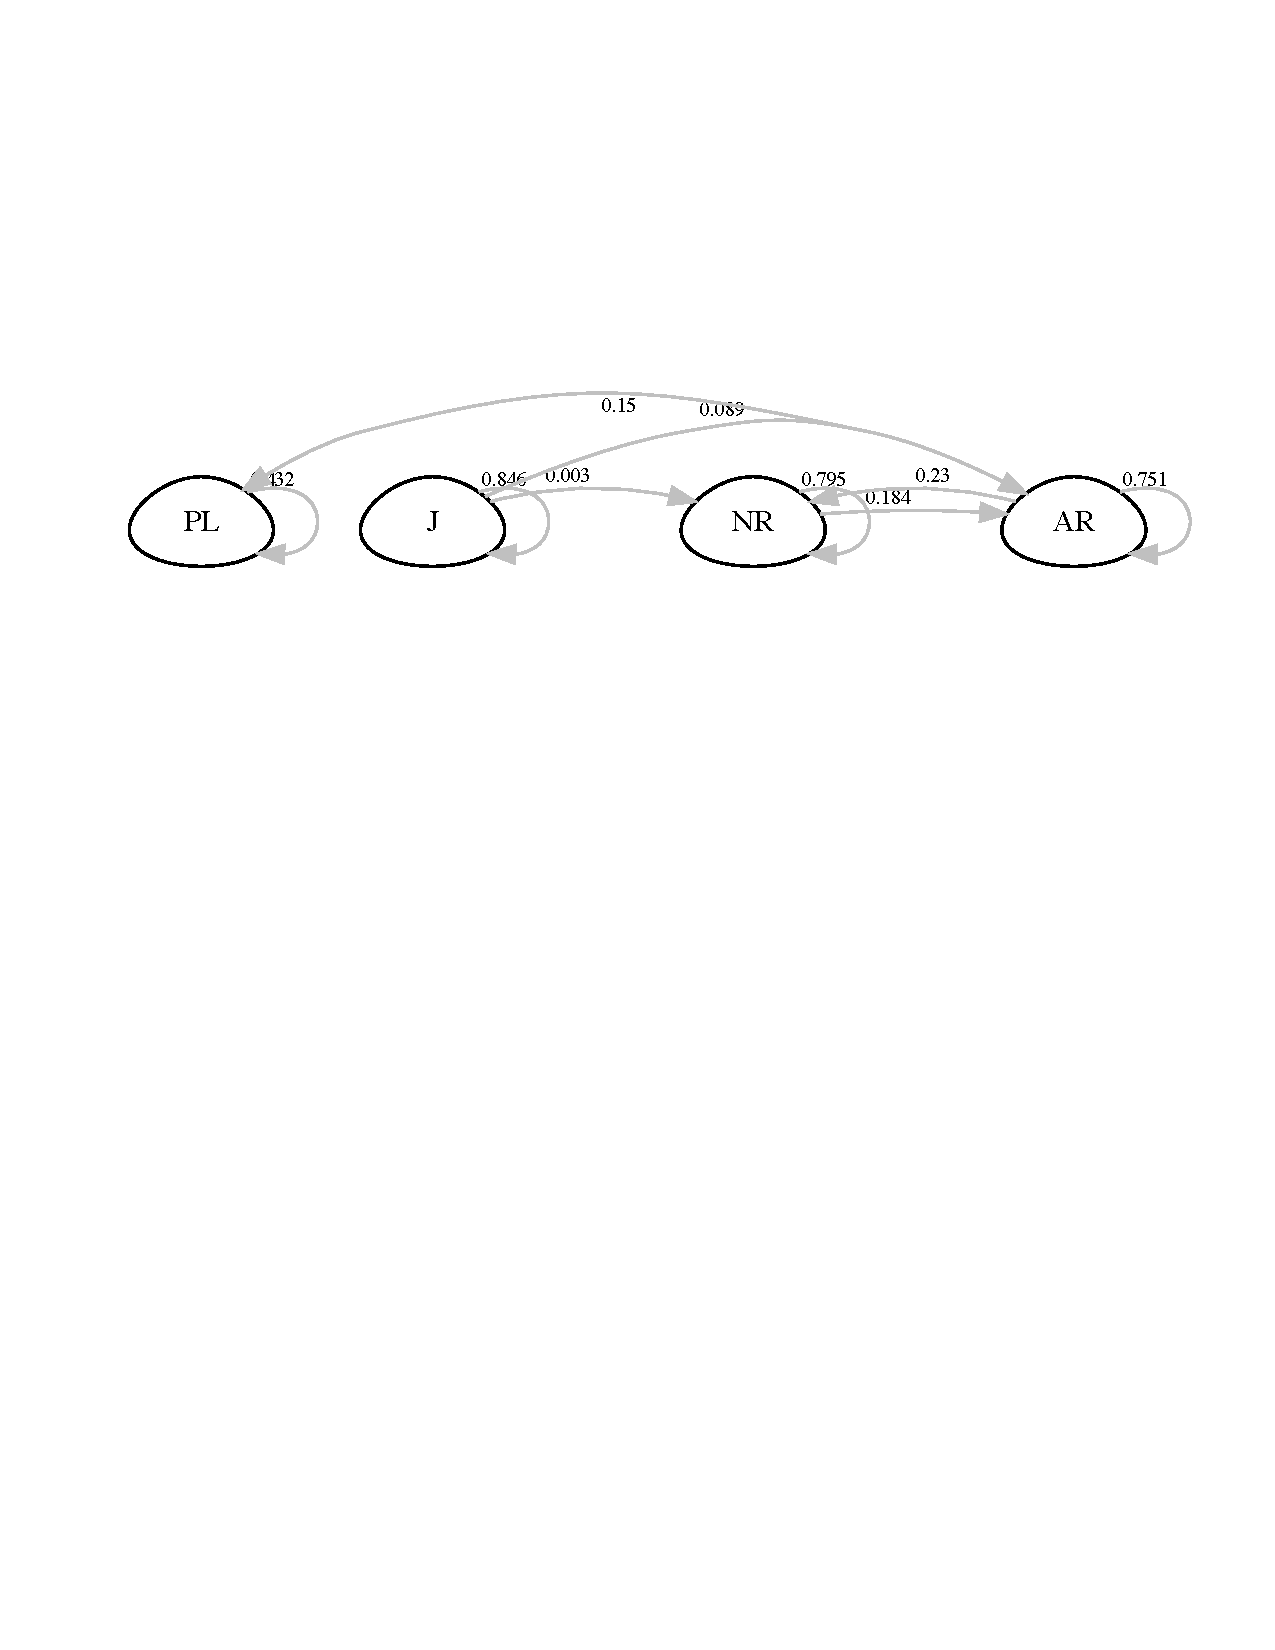
\includegraphics{110-Propriedades_files/figure-pdf/Indice5-1.pdf}

\begin{Shaded}
\begin{Highlighting}[]
\FunctionTok{isErgodic}\NormalTok{(Lr1\_No\_erg, }\AttributeTok{digits =} \DecValTok{4}\NormalTok{, }\AttributeTok{return.eigvec =} \ConstantTok{FALSE}\NormalTok{)}
\end{Highlighting}
\end{Shaded}

\begin{verbatim}
[1] FALSE
\end{verbatim}

\begin{center}\rule{0.5\linewidth}{0.5pt}\end{center}

\subsection{Elementos no negativa}\label{elementos-no-negativa}

Una matriz poblacional debe ser no negativa, lo que significa que todas
sus entradas son mayores o iguales a cero. ¿Por qué? Porque cada valor
representa el número o la proporción de individuos que pasan de una
etapa a otra. Tener valores negativos no tendría sentido biológico: no
puede haber ``menos'' individuos que los existentes.

Además, si la matriz tuviera elementos negativos:

\begin{itemize}
\tightlist
\item
  No podríamos comparar correctamente las categorías de edad o estado.
\item
  Sería imposible calcular la tasa de crecimiento poblacional.
\end{itemize}

En el caso de \emph{L. rubripetala}, la matriz cumple esta condición, ya
que todos sus valores son mayores o iguales a cero. En R, esto se puede
verificar con la función \texttt{isPositive}, que devuelve:

\begin{itemize}
\tightlist
\item
  TRUE si la matriz es no negativa,
\item
  FALSE si contiene algún valor negativo
\end{itemize}

\begin{Shaded}
\begin{Highlighting}[]
\CommentTok{\# No negativa }

\NormalTok{IsPositive }\OtherTok{\textless{}{-}} \ControlFlowTok{function}\NormalTok{(mat) \{}
  \ControlFlowTok{if}\NormalTok{ (}\FunctionTok{all}\NormalTok{(mat }\SpecialCharTok{\textgreater{}=} \DecValTok{0}\NormalTok{)) \{}
    \FunctionTok{return}\NormalTok{(}\ConstantTok{TRUE}\NormalTok{)}
\NormalTok{  \} }\ControlFlowTok{else}\NormalTok{ \{}
    \FunctionTok{return}\NormalTok{(}\ConstantTok{FALSE}\NormalTok{)}
\NormalTok{  \}}
\NormalTok{\}}

\FunctionTok{IsPositive}\NormalTok{(Lr1)}
\end{Highlighting}
\end{Shaded}

\begin{verbatim}
[1] TRUE
\end{verbatim}

A continuación se muestra un ejemplo de una matriz que no cumple la
propiedad de no negatividad. En este caso, el elemento ubicado en la
posición (4, 3) es negativo, lo que indica que la transición desde la
categoría adulto reproductivo hacia adulto no reproductivo tiene un
valor inválido.

Al evaluar esta matriz con la función \texttt{isPositive} en R, el
resultado es FALSE. Esto significa que:

\begin{itemize}
\tightlist
\item
  La matriz no es válida para el análisis de dinámica poblacional.
\item
  No se puede esperar que la población alcance una estructura estable ni
  una tasa de crecimiento constante a largo plazo.
\end{itemize}

\begin{Shaded}
\begin{Highlighting}[]
\CommentTok{\#Capturar los datos de la matriz para L. rubripetala (Tremblay et al. 2015)}
\NormalTok{Lr1\_No\_pos}\OtherTok{\textless{}{-}} \FunctionTok{matrix}\NormalTok{(}\FunctionTok{c}\NormalTok{(}\FloatTok{0.4324}\NormalTok{, }\DecValTok{0}\NormalTok{,      }\DecValTok{0}\NormalTok{,     }\FloatTok{0.15}\NormalTok{,}
               \FloatTok{0.3784}\NormalTok{, }\FloatTok{0.8459}\NormalTok{, }\DecValTok{0}\NormalTok{,     }\DecValTok{0}\NormalTok{,}
               \DecValTok{0}\NormalTok{,      }\FloatTok{0.0034}\NormalTok{, }\FloatTok{0.7954}\NormalTok{,}\SpecialCharTok{{-}}\FloatTok{0.2300}\NormalTok{,}
               \DecValTok{0}\NormalTok{,      }\FloatTok{0.0890}\NormalTok{, }\FloatTok{0.1841}\NormalTok{,}\FloatTok{0.7510}\NormalTok{), }\AttributeTok{byrow=}\ConstantTok{TRUE}\NormalTok{,}\AttributeTok{ncol=}\DecValTok{4}\NormalTok{)}



\FunctionTok{IsPositive}\NormalTok{(Lr1\_No\_pos)}
\end{Highlighting}
\end{Shaded}

\begin{verbatim}
[1] FALSE
\end{verbatim}

\begin{center}\rule{0.5\linewidth}{0.5pt}\end{center}

\subsection{Irreducibilidad}\label{irreducibilidad}

Una matriz de transición poblacional debe ser irreducible, lo que
significa que todas sus categorías están conectadas y existe al menos
una ruta que permite llegar desde cualquier estado a los demás. Esta
propiedad es esencial porque, si la matriz no es irreducible, la
población no podrá alcanzar una estructura estable ni una tasa de
crecimiento constante a largo plazo.

En el caso de \emph{L. rubripetala}, la matriz es irreducible: todas las
etapas del ciclo de vida están conectadas y existe una ruta entre ellas.
Para comprobar esta propiedad en R, se utiliza la función
\texttt{isIrreducible} del paquete popdemo, que devuelve:

\begin{itemize}
\tightlist
\item
  TRUE si la matriz es irreducible,
\item
  FALSE si no lo es.
\end{itemize}

Es importante destacar que no todas las matrices reducibles son
inválidas. En algunos casos, pueden aceptarse, por ejemplo, en especies
con etapas que no influyen en el crecimiento poblacional, como las fases
postreproductivas en mamíferos (humanos, ballenas, etc.).

En resumen, para \emph{L. rubripetala}, la función
\texttt{isIrreducible} devuelve TRUE, lo que confirma que todas las
categorías están conectadas y que la población puede alcanzar una
estructura estable y una tasa de crecimiento constante a largo plazo.

\begin{Shaded}
\begin{Highlighting}[]
\FunctionTok{isIrreducible}\NormalTok{(Lr1)}
\end{Highlighting}
\end{Shaded}

\begin{verbatim}
[1] TRUE
\end{verbatim}

A continuación se muestra un ejemplo de matriz en la que el cuarto
estadio no presenta valores de reproducción. Al evaluar esta matriz con
la función \texttt{isIrreducible} en R, el resultado es FALSE.

¿Por qué ocurre esto? Porque no existe un vínculo entre la categoría
plántula y la categoría adulto reproductivo, lo que significa que la
presencia de plántulas en la población no contribuye a la reproducción.

Esta ausencia de conexión provoca dos problemas:

\begin{itemize}
\tightlist
\item
  Un ciclo de vida incompleto, como se observa en la imagen.
\item
  Una población que no podrá alcanzar una estructura estable ni una tasa
  de crecimiento constante a largo plazo.
\end{itemize}

\begin{Shaded}
\begin{Highlighting}[]
\NormalTok{Lr1\_Irr }\OtherTok{\textless{}{-}} \FunctionTok{matrix}\NormalTok{(}\FunctionTok{c}\NormalTok{(}\FloatTok{0.4324}\NormalTok{,  }\FloatTok{0.}\NormalTok{,       }\FloatTok{0.0}\NormalTok{,     }\DecValTok{0}\NormalTok{,}
                    \FloatTok{0.3784}\NormalTok{,  }\FloatTok{0.8459}\NormalTok{,   }\DecValTok{0}\NormalTok{,       }\DecValTok{0}\NormalTok{,}
                    \FloatTok{0.}\NormalTok{,      }\FloatTok{0.0034}\NormalTok{,   }\FloatTok{0.7954}\NormalTok{,  }\FloatTok{0.2300}\NormalTok{,}
                    \DecValTok{0}\NormalTok{,       }\FloatTok{0.0890}\NormalTok{,   }\FloatTok{0.1841}\NormalTok{,  }\FloatTok{0.7510}\NormalTok{), }\AttributeTok{byrow=}\ConstantTok{TRUE}\NormalTok{,}\AttributeTok{ncol=}\DecValTok{4}\NormalTok{)}


\FunctionTok{plot\_life\_cycle}\NormalTok{(Lr1\_Irr, }\AttributeTok{stages =}\NormalTok{ estadios, }\AttributeTok{fontsize =} \DecValTok{8}\NormalTok{)}
\end{Highlighting}
\end{Shaded}

\begin{verbatim}
file:////private/var/folders/3k/1ft37x9130vdbz21tw1497x40000gn/T/RtmpOFXnC6/file1084e5eb4767e/widget1084e19cf7ac5.html screenshot completed
\end{verbatim}

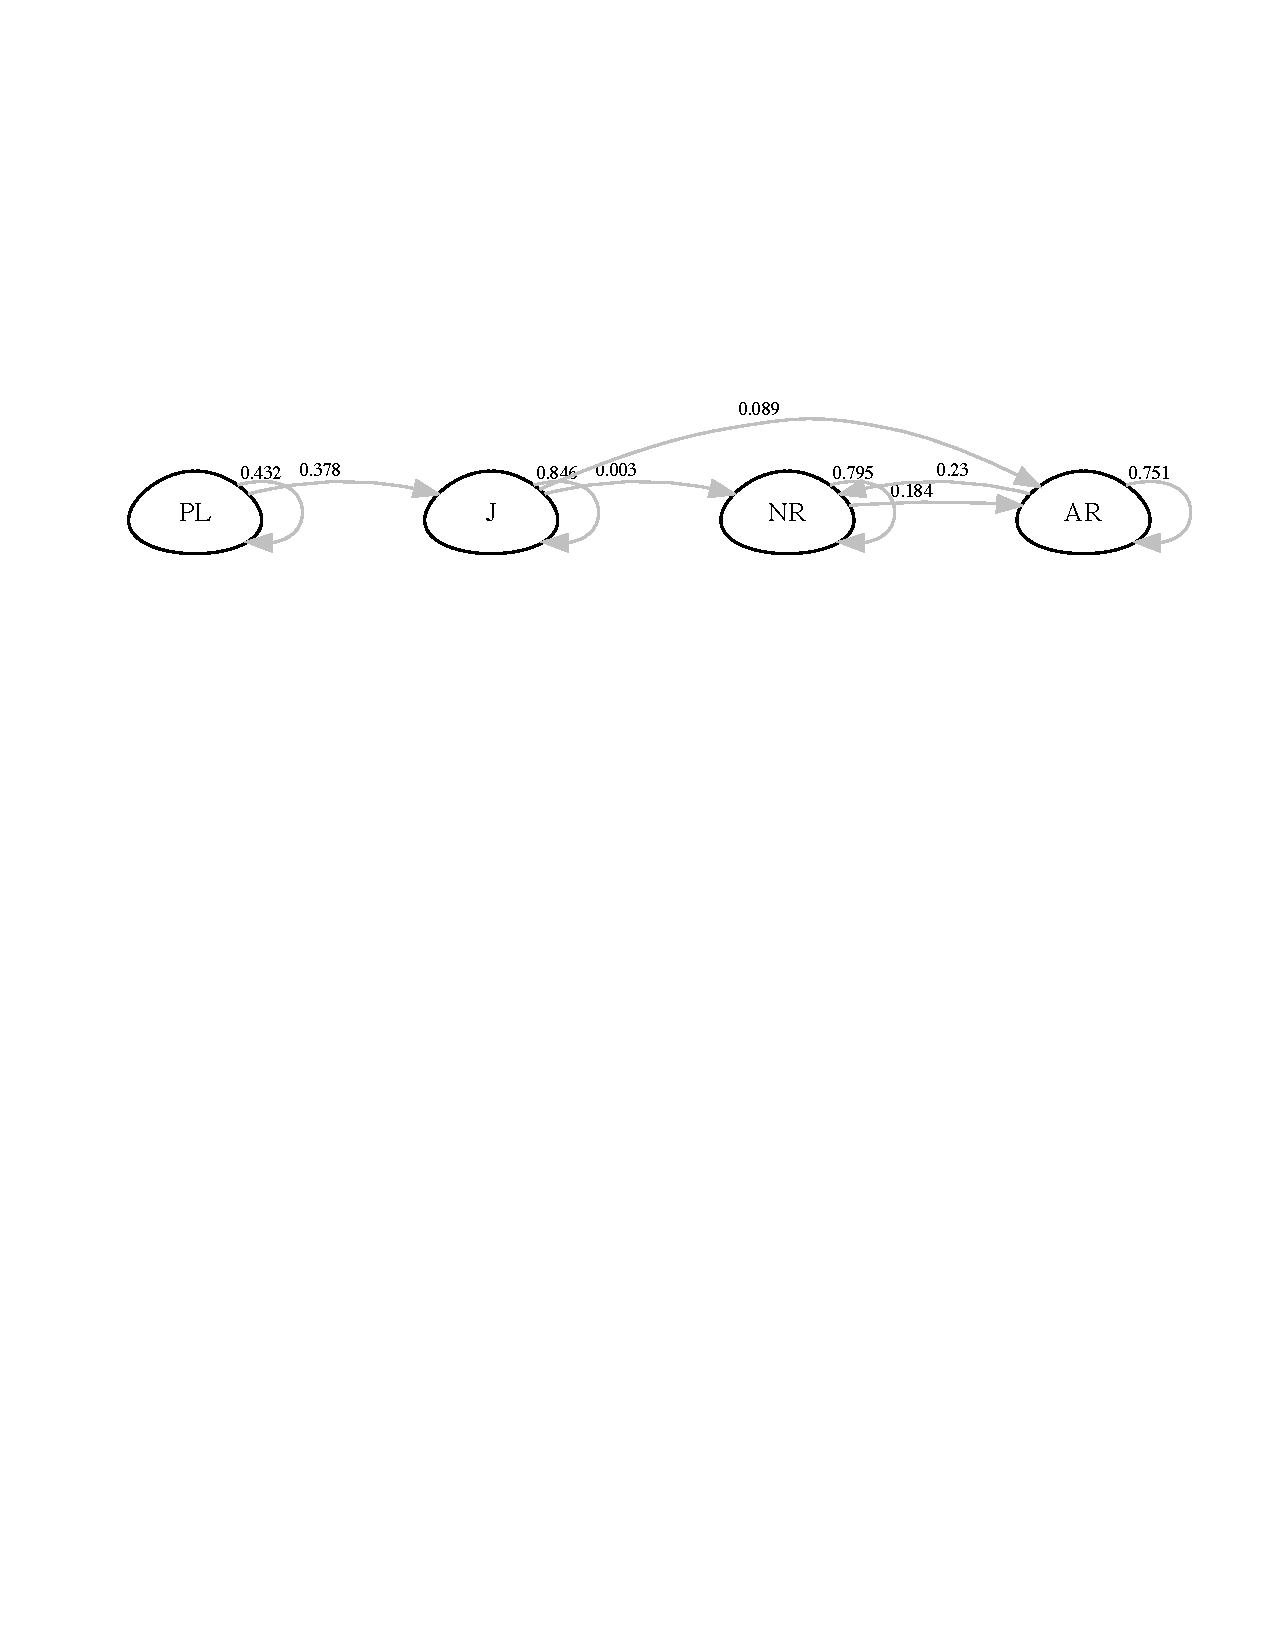
\includegraphics{110-Propriedades_files/figure-pdf/unnamed-chunk-2-1.pdf}

\begin{Shaded}
\begin{Highlighting}[]
\FunctionTok{isIrreducible}\NormalTok{(Lr1\_Irr)}
\end{Highlighting}
\end{Shaded}

\begin{verbatim}
[1] FALSE
\end{verbatim}

\begin{center}\rule{0.5\linewidth}{0.5pt}\end{center}

\subsection{Primitividad}\label{primitividad}

Una matriz de transición poblacional debe ser primitiva, lo que
significa que, al elevarla a potencias altas, se obtiene un único valor
positivo dominante (la tasa de crecimiento poblacional). Esta propiedad
es clave porque asegura que la población alcanzará una estructura
estable y una tasa de crecimiento constante a largo plazo.

En el caso de \emph{L. rubripetala}, la matriz es primitiva: al elevarla
a potencias altas, aparece un único valor positivo. En R, esto se puede
comprobar con la función \texttt{isPrimitive} del paquete popdemo, que
devuelve:

\begin{itemize}
\tightlist
\item
  TRUE si la matriz es primitiva,
\item
  FALSE si no lo es.
\end{itemize}

Una matriz no primitiva tendría una dinámica inestable a largo plazo,
como ocurre en poblaciones con comportamiento cíclico, donde las
proporciones entre categorías oscilan sin llegar a estabilizarse.

Es importante señalar que:

\begin{itemize}
\tightlist
\item
  Toda matriz irreducible es primitiva,
\item
  Pero no toda matriz primitiva es irreducible. Por ejemplo, una matriz
  puede ser primitiva sin ser irreducible si incluye un ciclo de vida
  completo, pero alguna etapa no influye en el crecimiento poblacional
  (como fases postreproductivas).
\end{itemize}

\begin{Shaded}
\begin{Highlighting}[]
\FunctionTok{isPrimitive}\NormalTok{(Lr1)}
\end{Highlighting}
\end{Shaded}

\begin{verbatim}
[1] TRUE
\end{verbatim}

\begin{center}\rule{0.5\linewidth}{0.5pt}\end{center}

\section{Índices de descripción de la matriz
poblacional}\label{uxedndices-de-descripciuxf3n-de-la-matriz-poblacional}

En esta sección se revisan los índices poblacionales obtenidos a partir
del análisis de matricial, los cuales se estiman una vez que ha
verificado que cumplen con los supuestos. Estos índices permiten
comprender el comportamiento de la población a largo plazo y anticipar
cómo se espera que se comporte en el tiempo. Los índices que se abordan
a continuación son: \textbf{estructura estable}, \textbf{valor
reproductivo}, \textbf{análisis de convergencia} y \textbf{análisis de
amortiguamiento}. Todos estos se calculan a partir de la matriz de
transición poblacional y del vector de la estructura poblacional
observada al inicio del estudio.

\begin{center}\rule{0.5\linewidth}{0.5pt}\end{center}

\subsection{Estructura Estable}\label{estructura-estable}

La estructura poblacional estable (W, también conocida como eigenvector
derecho) indica la proporción esperada de individuos en cada categoría
de edad o estado cuando la población ha alcanzado el equilibrio a largo
plazo. Por ejemplo, en L. rubripetala se espera que la estructura
estable sea:

\begin{itemize}
\tightlist
\item
  Plántulas: 0.088
\item
  Juveniles: 0.206
\item
  Adultos no reproductivos: 0.369
\item
  Adultos reproductivos: 0.337
\end{itemize}

Este índice supone que la tasa de crecimiento poblacional (\(\lambda\))
se mantiene constante en el tiempo, lo cual solo ocurre bajo condiciones
ambientales estables. Sin embargo, en la naturaleza esto es poco común.
Además, la estructura estable asume que el periodo de muestreo y las
condiciones abióticas y bióticas son típicas y no cambian.

En la revisión de Williams y colaboradores (Williams et al., 2011), se
reportó que más del 80\% de las poblaciones analizadas no cumplían con
la condición de estructura estable, especialmente en especies con
matrices grandes (n × n) y tiempos generacionales prolongados. De manera
similar, Tremblay (com. pers.) observó que la mayoría de las orquídeas
estudiadas no estaban en estructura estable al inicio del muestreo
poblacional.

\begin{Shaded}
\begin{Highlighting}[]
\CommentTok{\#Estructura estable de estados}

\FunctionTok{stable.stage}\NormalTok{(Lr1)}
\end{Highlighting}
\end{Shaded}

\begin{verbatim}
        PL          J         NR         AR 
0.08789851 0.20619682 0.36907404 0.33683063 
\end{verbatim}

Uno puede visualizar la estructura poblacional usando el código
siguiente.

\begin{Shaded}
\begin{Highlighting}[]
\NormalTok{Wmax }\OtherTok{\textless{}{-}} \FunctionTok{stable.stage}\NormalTok{(Lr1)}
\NormalTok{Wdf }\OtherTok{=} \FunctionTok{data.frame}\NormalTok{(Wmax)}
\NormalTok{Wdf}\SpecialCharTok{$}\NormalTok{Categorias }\OtherTok{=} \FunctionTok{c}\NormalTok{(}
  \StringTok{"Plántulas"}\NormalTok{,}
  \StringTok{"Juveniles"}\NormalTok{,}
  \StringTok{"Adultos no reproductivos"}\NormalTok{,}
  \StringTok{"Adultos reproductivos"}
\NormalTok{)}
\NormalTok{Wdf}\SpecialCharTok{$}\NormalTok{Categorias }\OtherTok{=} \FunctionTok{factor}\NormalTok{(}
\NormalTok{  Wdf}\SpecialCharTok{$}\NormalTok{Categorias,}
  \AttributeTok{levels =} \FunctionTok{c}\NormalTok{(}
    \StringTok{"Plántulas"}\NormalTok{,}
    \StringTok{"Juveniles"}\NormalTok{,}
    \StringTok{"Adultos no reproductivos"}\NormalTok{,}
    \StringTok{"Adultos reproductivos"}
\NormalTok{  )}
\NormalTok{)}
\FunctionTok{library}\NormalTok{(ggplot2)}

\FunctionTok{ggplot}\NormalTok{(Wdf, }\FunctionTok{aes}\NormalTok{(}\AttributeTok{y =}\NormalTok{ Wmax, }\AttributeTok{x =}\NormalTok{ Categorias)) }\SpecialCharTok{+}
  \FunctionTok{geom\_bar}\NormalTok{(}\AttributeTok{stat =} \StringTok{"identity"}\NormalTok{, }\FunctionTok{aes}\NormalTok{(}\AttributeTok{fill =} \StringTok{"blue"}\NormalTok{)) }\SpecialCharTok{+}
  \FunctionTok{labs}\NormalTok{(}
    \AttributeTok{title =} \StringTok{"Estructura estable de estados esperada"}\NormalTok{,}
    \AttributeTok{x =} \StringTok{"Etapas"}\NormalTok{,}
    \AttributeTok{y =} \StringTok{"Proporción"}
\NormalTok{  ) }\SpecialCharTok{+}
  \FunctionTok{rlt\_style\_fill}\NormalTok{()}\SpecialCharTok{+}
  \FunctionTok{theme}\NormalTok{(}\AttributeTok{axis.text.x =} \FunctionTok{element\_text}\NormalTok{(}\AttributeTok{angle =} \DecValTok{45}\NormalTok{, }\AttributeTok{hjust =} \DecValTok{1}\NormalTok{))}\SpecialCharTok{+}
  \FunctionTok{theme}\NormalTok{(}\AttributeTok{legend.position=}\StringTok{"null"}\NormalTok{)}
\end{Highlighting}
\end{Shaded}

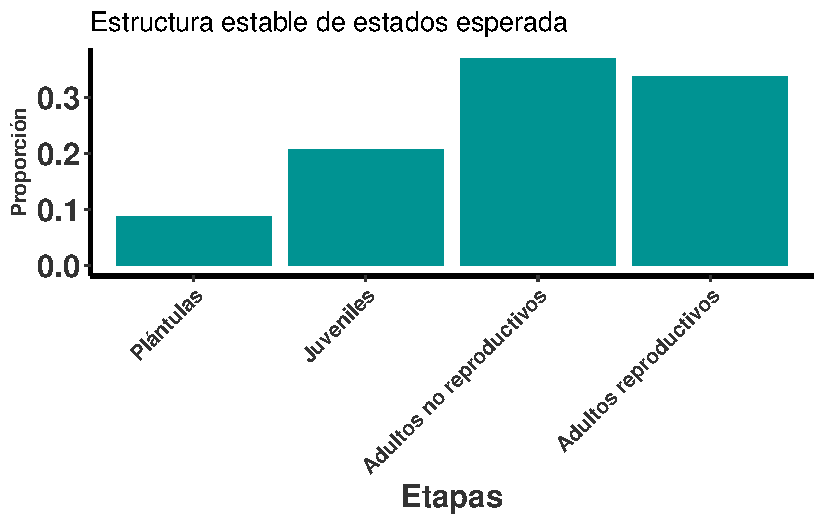
\includegraphics{110-Propriedades_files/figure-pdf/Indice10-1.pdf}

\begin{center}\rule{0.5\linewidth}{0.5pt}\end{center}

\subsection{Valor reproductivo}\label{valor-reproductivo}

\begin{figure}[H]

{\centering 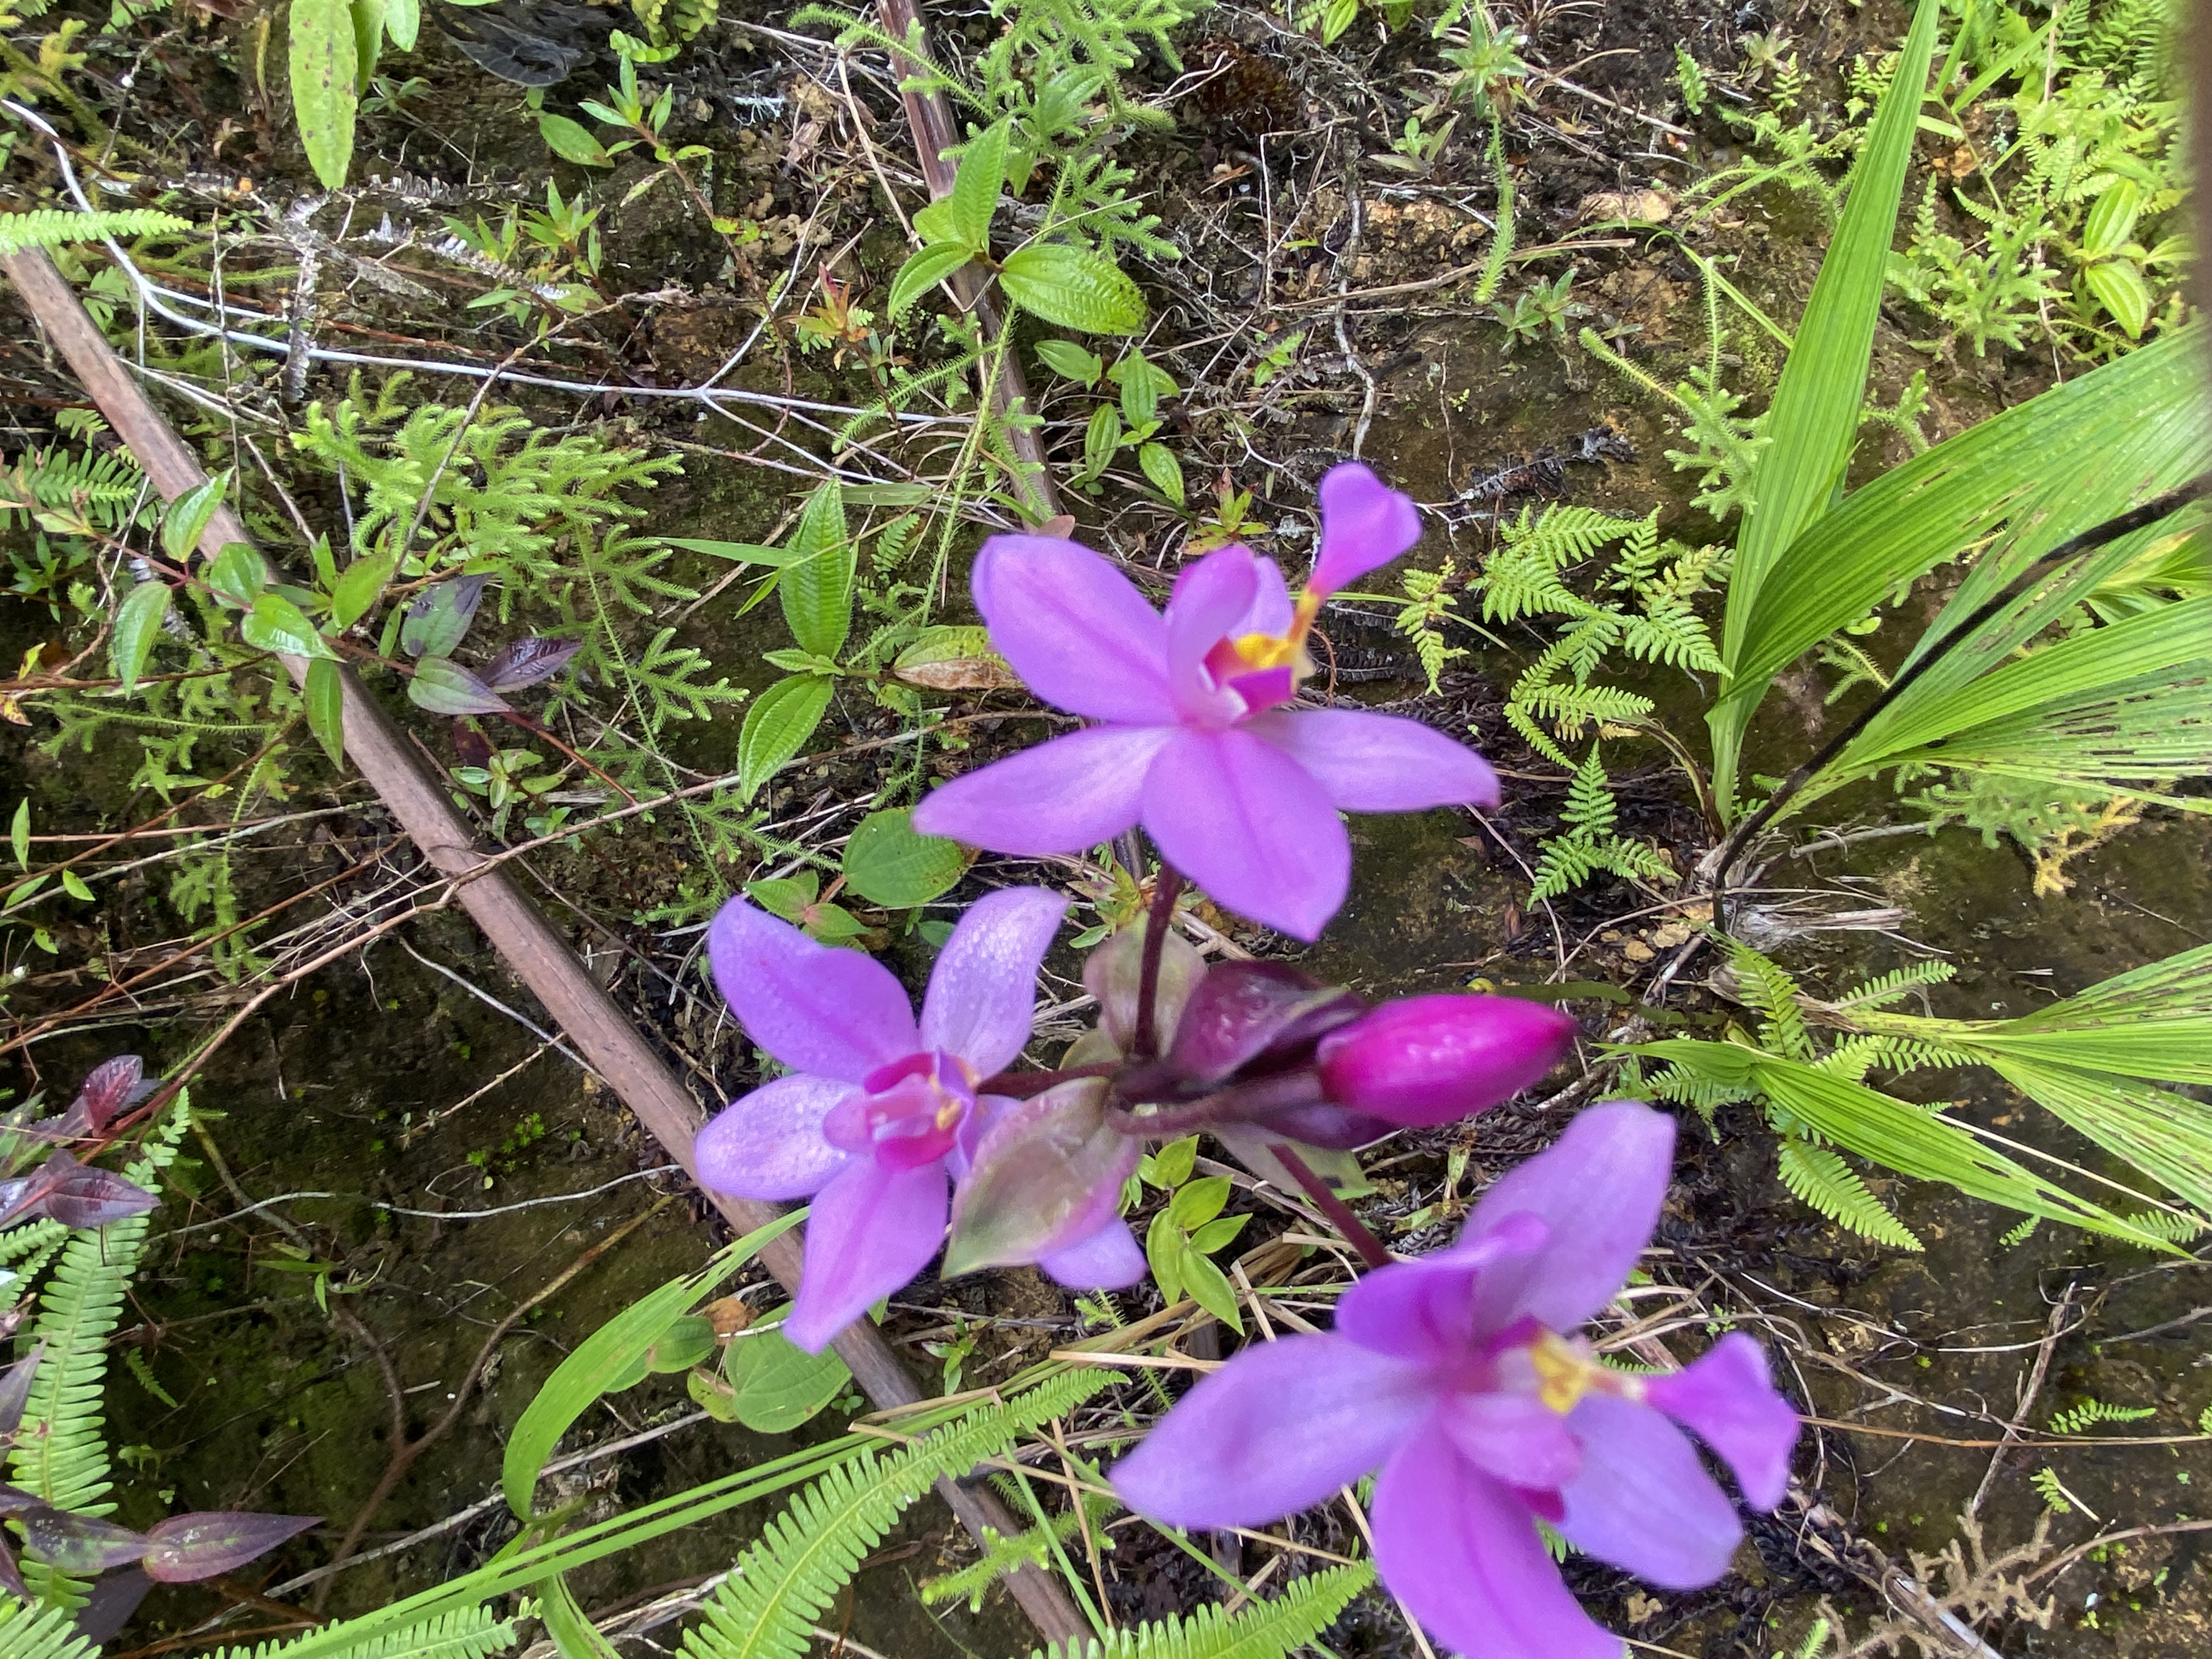
\includegraphics{Species/Spathoglottis plicata Tremblay.jpeg}

}

\caption{\emph{Spathoglottis plicata}. Foto: Tremblay}

\end{figure}%

El valor reproductivo (v, también llamado eigenvector izquierdo) indica
la contribución esperada de cada categoría de edad o estado a la
reproducción de la población.

En el caso de L. rubripetala, los valores reproductivos esperados son:

\begin{itemize}
\tightlist
\item
  Plántulas: 1.00
\item
  Juveniles: 1.52
\item
  Adultos no reproductivos: 2.32
\item
  Adultos reproductivos: 2.66
\end{itemize}

Este índice es muy útil porque muestra qué etapas son más importantes
para el crecimiento poblacional a largo plazo. La primera categoría
siempre tiene un valor de 1.00, ya que representa el inicio del ciclo de
vida y sirve como referencia para calcular los demás valores.

Además, el valor reproductivo ayuda a definir estrategias de manejo. Por
ejemplo:

\begin{itemize}
\item
  En \emph{Spathoglottis plicata}, una orquídea terrestre invasora, las
  acciones de control deberían enfocarse en las categorías con mayor
  valor reproductivo, porque son las que más contribuyen al crecimiento
  poblacional.
\item
  Por el contrario, si se busca remover individuos con el menor impacto
  posible, conviene actuar sobre las etapas con valores reproductivos
  bajos.
\end{itemize}

\begin{Shaded}
\begin{Highlighting}[]
\CommentTok{\# Valor reproductivo}

\FunctionTok{reproductive.value}\NormalTok{(Lr1)}
\end{Highlighting}
\end{Shaded}

\begin{verbatim}
      PL        J       NR       AR 
1.000000 1.519043 2.316113 2.664676 
\end{verbatim}

\begin{center}\rule{0.5\linewidth}{0.5pt}\end{center}

\subsection{Análisis de Convergencia y Amortigamiento (Damping
ratio)}\label{anuxe1lisis-de-convergencia-y-amortigamiento-damping-ratio}

El análisis de convergencia mide el tiempo esperado para que una
población alcance su estructura estable y un crecimiento asintótico
después de un disturbio. Es decir, indica qué tan rápido la población
regresa a su estructura estable tras una perturbación (Stott, Townley \&
Hodgson, 2011). Este comportamiento se cuantifica mediante el índice de
amortiguamiento (damping ratio), que evalúa la influencia del valor
propio subdominante, \(\lambda_2\), durante el periodo de convergencia.

El índice se expresa a través del cociente entre el valor propio
dominante, \(\lambda_1\), y el valor absoluto del subdominante
\[\mathbf{\rho=\frac{\lambda_1}{\left|\lambda_2\right|}}\]; dónde
\(\rho\) representa el índice de amortiguamiento, \(\lambda_1\)
corresponde al valor propio dominante de la matriz de transición
poblacional y \(\lambda_2\) al módulo del segundo valor propio más
grande. Este índice no tiene unidades y es independiente de la
estructura inicial de la población.

En el caso de \emph{L. rubripetala}, al calcular los valores propios de
la matriz con la función \textbf{eigen}, se obtiene un valor dominante
de \(\lambda_1= 1.00721\) y un valor subdominante de
\(\lambda_2= 0.8319\). De esta manera el índice de amortiguamiento es:

\[
\rho = \frac{\lambda_1}{|\lambda_2|} = \frac{1.00721}{|0.83192|} \approx 1.21
\]

El valor obtenido indica que la población converge hacia su estructura
estable tras un disturbio; aunque, lentamente.

Es importante señalar que la interpretación de este índice depende de la
escala temporal con que se construyó la matriz. Si bien la mayoría de
los estudios poblacionales utilizan datos anuales (Crone et al., 2011),
también existen estudios con periodos de muestreo mensuales,
bimensuales, estacionales o bianuales, los cuales se establecen de
acuerdo con el ciclo de vida de la especie estudiada.

\begin{Shaded}
\begin{Highlighting}[]
\FunctionTok{eigen}\NormalTok{(Lr1)}\SpecialCharTok{$}\NormalTok{values }\CommentTok{\# la lista de valores propios de la matriz Lr1}
\end{Highlighting}
\end{Shaded}

\begin{verbatim}
[1] 1.0072061+0.00000000i 0.8319189+0.00000000i 0.4927875+0.06468183i
[4] 0.4927875-0.06468183i
\end{verbatim}

\begin{Shaded}
\begin{Highlighting}[]
\NormalTok{DR }\OtherTok{=} \FunctionTok{eigen}\NormalTok{(Lr1)}\SpecialCharTok{$}\NormalTok{values[}\DecValTok{1}\NormalTok{] }\SpecialCharTok{/} \FunctionTok{abs}\NormalTok{(}\FunctionTok{eigen}\NormalTok{(Lr1)}\SpecialCharTok{$}\NormalTok{values[}\DecValTok{2}\NormalTok{])}

\NormalTok{DR}
\end{Highlighting}
\end{Shaded}

\begin{verbatim}
[1] 1.210702+0i
\end{verbatim}

\begin{Shaded}
\begin{Highlighting}[]
\FunctionTok{dr}\NormalTok{(Lr1) }\CommentTok{\# usando la función "dr" para "damping ratio" en el paquete "popdemo"}
\end{Highlighting}
\end{Shaded}

\begin{verbatim}
[1] 1.210702
\end{verbatim}

\subsection{Graficación del Índice de
amortiguamiento}\label{graficaciuxf3n-del-uxedndice-de-amortiguamiento}

El comportamiento del índice de amortiguamiento se puede visualizar
mediante una gráfica de líneas, que muestra cómo responde un sistema
ante un cambio súbito (un ``paso de entrada'') y cómo varía esa
respuesta en el tiempo según diferentes niveles de amortiguamiento.

Para facilitar la comprensión, en el siguiente bloque se incluye el
código que genera una gráfica ilustrando el comportamiento de una
población perturbada:

\begin{Shaded}
\begin{Highlighting}[]
\FunctionTok{library}\NormalTok{(ggplot2)}

\CommentTok{\# {-}{-}{-} Definir los parametros {-}{-}{-}}
\CommentTok{\# Población inicial en el tiempo t=0. Ese el punto de equilibrio inicial.}
\NormalTok{poblacion\_inicial }\OtherTok{\textless{}{-}} \DecValTok{1000}

\CommentTok{\# Factores de amortiguamiento para graficar.}
\CommentTok{\# 0,3 = Subamortiguado (oscila)}
\CommentTok{\# 1,0 = Críticamente amortiguado (retorno más rápido sin oscilación)}
\CommentTok{\# 2,0 = Sobreamortiguado (retorno lento sin oscilación)}
\NormalTok{amortigamento }\OtherTok{\textless{}{-}} \FunctionTok{c}\NormalTok{(}\FloatTok{0.3}\NormalTok{, }\FloatTok{1.0}\NormalTok{, }\FloatTok{2.0}\NormalTok{, }\FloatTok{3.0}\NormalTok{)}

\CommentTok{\# Frecuencia de la oscilación (omega\_n).}
\NormalTok{frecuencia }\OtherTok{\textless{}{-}} \FloatTok{0.5}

\CommentTok{\# Tiempo total para la simulación}
\NormalTok{tiempo\_total }\OtherTok{\textless{}{-}} \DecValTok{50}

\CommentTok{\# Paso de tiempo para la simulación (más pequeño para una curva más suave)}
\NormalTok{etapa\_tiempo }\OtherTok{\textless{}{-}} \FloatTok{0.1}

\CommentTok{\# {-}{-}{-} Generate the Damped Oscillation Data for Multiple Ratios {-}{-}{-}}
\CommentTok{\# Create an empty data frame to store all the data}
\NormalTok{todo\_data\_df }\OtherTok{\textless{}{-}} \FunctionTok{data.frame}\NormalTok{()}

\CommentTok{\# Recorra cada relación de amortiguamiento para generar los datos}
\ControlFlowTok{for}\NormalTok{ (zeta }\ControlFlowTok{in}\NormalTok{ amortigamento) \{}
  \CommentTok{\# Create a sequence of time points}
\NormalTok{  time\_points }\OtherTok{\textless{}{-}} \FunctionTok{seq}\NormalTok{(}\DecValTok{0}\NormalTok{, tiempo\_total, }\AttributeTok{by =}\NormalTok{ etapa\_tiempo)}

  \CommentTok{\# Calculate the population at each time point based on the damping ratio.}
  \CommentTok{\# The mathematical form of the step response changes depending on the damping ratio.}

  \ControlFlowTok{if}\NormalTok{ (zeta }\SpecialCharTok{\textless{}} \DecValTok{1}\NormalTok{) \{}
    \CommentTok{\# Underdamped case: damped sine wave}
\NormalTok{    omega\_d }\OtherTok{\textless{}{-}}\NormalTok{ frecuencia }\SpecialCharTok{*} \FunctionTok{sqrt}\NormalTok{(}\DecValTok{1} \SpecialCharTok{{-}}\NormalTok{ zeta}\SpecialCharTok{\^{}}\DecValTok{2}\NormalTok{)}
\NormalTok{    population\_data }\OtherTok{\textless{}{-}}\NormalTok{ poblacion\_inicial }\SpecialCharTok{*}
\NormalTok{      (}\DecValTok{1} \SpecialCharTok{{-}}
        \FunctionTok{exp}\NormalTok{(}\SpecialCharTok{{-}}\NormalTok{zeta }\SpecialCharTok{*}\NormalTok{ frecuencia }\SpecialCharTok{*}\NormalTok{ time\_points) }\SpecialCharTok{*}
\NormalTok{          (}\FunctionTok{cos}\NormalTok{(omega\_d }\SpecialCharTok{*}\NormalTok{ time\_points) }\SpecialCharTok{+}
\NormalTok{            (zeta }\SpecialCharTok{/} \FunctionTok{sqrt}\NormalTok{(}\DecValTok{1} \SpecialCharTok{{-}}\NormalTok{ zeta}\SpecialCharTok{\^{}}\DecValTok{2}\NormalTok{)) }\SpecialCharTok{*} \FunctionTok{sin}\NormalTok{(omega\_d }\SpecialCharTok{*}\NormalTok{ time\_points)))}
\NormalTok{  \} }\ControlFlowTok{else} \ControlFlowTok{if}\NormalTok{ (zeta }\SpecialCharTok{==} \DecValTok{1}\NormalTok{) \{}
    \CommentTok{\# Critically Damped case}
\NormalTok{    population\_data }\OtherTok{\textless{}{-}}\NormalTok{ poblacion\_inicial }\SpecialCharTok{*}
\NormalTok{      (}\DecValTok{1} \SpecialCharTok{{-}} \FunctionTok{exp}\NormalTok{(}\SpecialCharTok{{-}}\NormalTok{frecuencia }\SpecialCharTok{*}\NormalTok{ time\_points) }\SpecialCharTok{*}\NormalTok{ (}\DecValTok{1} \SpecialCharTok{+}\NormalTok{ frecuencia }\SpecialCharTok{*}\NormalTok{ time\_points))}
\NormalTok{  \} }\ControlFlowTok{else}\NormalTok{ \{}
    \CommentTok{\# Overdamped case}
\NormalTok{    s1 }\OtherTok{\textless{}{-}} \SpecialCharTok{{-}}\NormalTok{zeta }\SpecialCharTok{*}\NormalTok{ frecuencia }\SpecialCharTok{+}\NormalTok{ frecuencia }\SpecialCharTok{*} \FunctionTok{sqrt}\NormalTok{(zeta}\SpecialCharTok{\^{}}\DecValTok{2} \SpecialCharTok{{-}} \DecValTok{1}\NormalTok{)}
\NormalTok{    s2 }\OtherTok{\textless{}{-}} \SpecialCharTok{{-}}\NormalTok{zeta }\SpecialCharTok{*}\NormalTok{ frecuencia }\SpecialCharTok{{-}}\NormalTok{ frecuencia }\SpecialCharTok{*} \FunctionTok{sqrt}\NormalTok{(zeta}\SpecialCharTok{\^{}}\DecValTok{2} \SpecialCharTok{{-}} \DecValTok{1}\NormalTok{)}
\NormalTok{    population\_data }\OtherTok{\textless{}{-}}\NormalTok{ poblacion\_inicial }\SpecialCharTok{*}
\NormalTok{      (}\DecValTok{1} \SpecialCharTok{{-}}
\NormalTok{        (s2 }\SpecialCharTok{*} \FunctionTok{exp}\NormalTok{(s1 }\SpecialCharTok{*}\NormalTok{ time\_points) }\SpecialCharTok{{-}}\NormalTok{ s1 }\SpecialCharTok{*} \FunctionTok{exp}\NormalTok{(s2 }\SpecialCharTok{*}\NormalTok{ time\_points)) }\SpecialCharTok{/}\NormalTok{ (s2 }\SpecialCharTok{{-}}\NormalTok{ s1))}
\NormalTok{  \}}

  \CommentTok{\# Add the data for the current damping ratio to a temporary data frame}
\NormalTok{  temp\_df }\OtherTok{\textless{}{-}} \FunctionTok{data.frame}\NormalTok{(}
    \AttributeTok{Time =}\NormalTok{ time\_points,}
    \AttributeTok{Population =}\NormalTok{ population\_data,}
    \AttributeTok{DampingRatio =} \FunctionTok{factor}\NormalTok{(zeta) }\CommentTok{\# Store damping ratio as a factor for coloring}
\NormalTok{  )}

  \CommentTok{\# Bind the temporary data frame to the main data frame}
\NormalTok{  todo\_data\_df }\OtherTok{\textless{}{-}} \FunctionTok{rbind}\NormalTok{(todo\_data\_df, temp\_df)}
\NormalTok{\}}

\CommentTok{\# {-}{-}{-} Create the Plot using ggplot2 {-}{-}{-}}
\FunctionTok{ggplot}\NormalTok{(todo\_data\_df, }\FunctionTok{aes}\NormalTok{(}\AttributeTok{x =}\NormalTok{ Time, }\AttributeTok{y =}\NormalTok{ Population, }\AttributeTok{color =}\NormalTok{ DampingRatio)) }\SpecialCharTok{+}
  \CommentTok{\# Add the lines for each damping ratio}
  \FunctionTok{geom\_line}\NormalTok{(}\AttributeTok{linewidth =} \FloatTok{1.2}\NormalTok{) }\SpecialCharTok{+}
  \CommentTok{\# Set the title and labels}
  \FunctionTok{labs}\NormalTok{(}
    \AttributeTok{title =} \StringTok{"El efecto de amortigamento }\SpecialCharTok{\textbackslash{}n}\StringTok{ sobre el tamaño de población"}\NormalTok{,}
    \AttributeTok{subtitle =} \StringTok{"La población se estabiliza a un equilibrio de 1000"}\NormalTok{,}
    \AttributeTok{x =} \StringTok{"Tiempo"}\NormalTok{,}
    \AttributeTok{y =} \StringTok{"Tamaño poblacional"}\NormalTok{,}
    \AttributeTok{color =} \StringTok{"Amortigamento (ζ)"} \CommentTok{\# Title for the legend}
\NormalTok{  ) }\SpecialCharTok{+}
  \CommentTok{\# Customize the plot theme for better aesthetics}
  \FunctionTok{rlt\_style\_colour}\NormalTok{() }\SpecialCharTok{+}
  \FunctionTok{theme\_minimal}\NormalTok{(}\AttributeTok{base\_size =} \DecValTok{14}\NormalTok{) }\SpecialCharTok{+}
  \FunctionTok{theme}\NormalTok{(}
    \AttributeTok{plot.title =} \FunctionTok{element\_text}\NormalTok{(}\AttributeTok{hjust =} \FloatTok{0.5}\NormalTok{, }\AttributeTok{face =} \StringTok{"bold"}\NormalTok{),}
    \AttributeTok{plot.subtitle =} \FunctionTok{element\_text}\NormalTok{(}\AttributeTok{hjust =} \FloatTok{0.5}\NormalTok{),}
    \AttributeTok{axis.title =} \FunctionTok{element\_text}\NormalTok{(}\AttributeTok{face =} \StringTok{"bold"}\NormalTok{)}
\NormalTok{  )}
\end{Highlighting}
\end{Shaded}

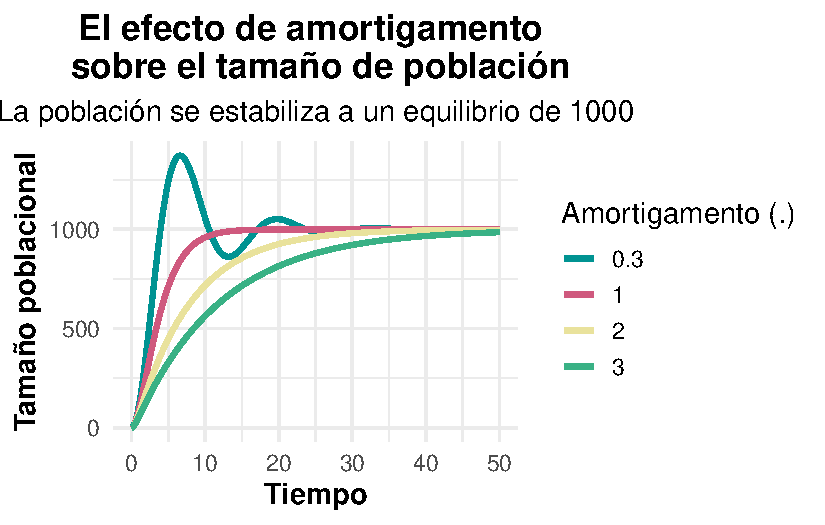
\includegraphics{110-Propriedades_files/figure-pdf/Indice13-1.pdf}

\subsection{Intepretación del gráfico de
amortiguamiento}\label{intepretaciuxf3n-del-gruxe1fico-de-amortiguamiento}

La figura resultante ilustra el efecto de diferentes coeficientes de
amortiguamiento en la respuesta de una población a un cambio súbito. El
gráfico muestra cuatro comportamientos distintos para la población
perturbada y su retorno a un estado de equilibrio, correspondiente a un
tamaño poblacional de 1000 individuos.

La respuesta de la población ante cuatro índices de amortiguamiento es
la siguiente:

• Subamortiguado (ζ=0.3): Esta es la respuesta oscilante. El sistema
sobrepasa el punto de equilibrio y luego oscila, con el tiempo la
amplitud de las oscilaciones disminuyen gradualmente hasta estabilizarse
en el equilibrio.

• Amortiguado críticamente (ζ=1.0): Esta es la respuesta más rápida, la
cual alcanza el equilibrio sin oscilaciones ni sobreamortiguaciones. Se
considera la respuesta ideal para sistemas que requieren un retorno
rápido y estable al valor objetivo.

• Sobreamortiguado (ζ=2.0): Esta respuesta es lenta y se aproxima al
punto de equilibrio sin oscilaciones. En comparación con el caso
críticamente amortiguado, tarda mucho más en estabilizarse, ya que la
fuerza de amortiguamiento es muy grande.

• Sobreamortiguado (ζ=3.0): Similar al caso anterior, pero con un
amortiguamiento aún mayor. La respuesta es muy lenta y se acerca al
equilibrio de manera gradual sin oscilaciones.

\subsubsection{Tiempo de Convergencia}\label{tiempo-de-convergencia}

El tiempo de convergencia es el periodo estimado que tarda la población
en alcanzar su estructura estable. Este índice es relevante porque
facilita entender el comportamiento poblacional a largo plazo. En
\textbf{R} este cálculo puede realizarse con dos funciones del paquete
\textbf{popdemo}: \textbf{dr} y \textbf{convt}. La función \textbf{dr}
calcula el amortiguamiento y a partir de éste puede estimarse el tiempo
de la convergencia de la siguiente manera:

\[
t = \frac{\log(dr)}{\log(x)}
\]

dónde

\begin{itemize}
\tightlist
\item
  \(dr\) es el índice de amortiguamiento (damping ratio)
\item
  \(x\) es un factor de comparación
\item
  \(t\) representa el tiempo en la misma unidad en que se construyó la
  matriz (días, meses, años, etc.).
\end{itemize}

El análisis de amortiguamiento estima la rapidez con la que una
población converge a su estructura estable después de un disturbio
(Jiang et al., 2020). El índice de amortiguamiento (\(d > 0\)) sugiere
que mientras mayor sea su valor, más rápida será la convergencia. El
tiempo de amortiguamiento se calcula como: \(\tau=1/d\), dónde \(\tau\)
expresa la duración del proceso de convergencia en unidades de tiempo
consistentes con la matriz poblacional. Cabe señalar que, se ha
demostrado que existe una relación entre el índice de amortiguamiento y
el tiempo generacional de una especie (Jiang et al., 2020).

\begin{Shaded}
\begin{Highlighting}[]
\FunctionTok{dr}\NormalTok{(Lr1, }\AttributeTok{return.time =} \ConstantTok{TRUE}\NormalTok{, }\AttributeTok{x =} \DecValTok{10}\NormalTok{) }\CommentTok{\# cuanto tiempo toma aumentar la población de veces }
\end{Highlighting}
\end{Shaded}

\begin{verbatim}
$dr
[1] 1.210702

$t
[1] 12.04278
\end{verbatim}

A partir de la la función \(contv\) del paquete \textbf{popdemo} se
puede estimar el tiempo esperado en que una población alcanza su
estructura estable, considerando la estructura poblacional observada al
inicio del estudio. Esta función simula el modelo y determina
manualmente cuándo la población converge, dado un nivel de exactitud
especifico (\emph{accuracy}). Entre más estricta sea la exactitud, mayor
será el tiempo de convergencia. Para utilizar esta función es necesario
indicar la estructura inicial, es decir, el número de individuos en cada
estadio. En el caso de \emph{L. rubripetala} se espera que el tiempo de
convergencia sea de 18 ciclos (meses) para alcanzar su estructura
estable.

Por ejemplo, si se comienza con una población inicial de 8, 20, 27 y 34
individuos en las categorías de plántulas, juveniles, adultos no
reproductivos y adultos reproductivos, respectivamente, la población
alcanzaría en 6 meses, aproximadamente, la estructura estable. En
contraste, si la población inicial estuviera sesgada (compuesta
únicamente por plántulas, por ejemplo), el tiempo de convergencia sería
mucho mayor. Este enfoque resulta muy útil al definir estrategias de
conservación; por ejemplo, al establecer una nueva población con una
distribución inicial determinada.

\begin{Shaded}
\begin{Highlighting}[]
\NormalTok{n0 }\OtherTok{\textless{}{-}} \FunctionTok{c}\NormalTok{(}\DecValTok{8}\NormalTok{, }\DecValTok{20}\NormalTok{, }\DecValTok{27}\NormalTok{, }\DecValTok{34}\NormalTok{) }\CommentTok{\# la estructura de la población inicial}

\FunctionTok{convt}\NormalTok{(Lr1, }\AttributeTok{accuracy =} \FloatTok{1e{-}4}\NormalTok{, }\AttributeTok{vector =}\NormalTok{ n0, }\AttributeTok{iterations =} \DecValTok{10000}\NormalTok{) }\CommentTok{\# la estructura poblacional inicial}
\end{Highlighting}
\end{Shaded}

\begin{verbatim}
[1] 18
\end{verbatim}

Dado que el tiempo de convergencia es un índice que representa el
periodo esperado para que una población alcance su estructura estable,
se puede calcular variando la cantidad de individuos en las diferentes
edades o estados al llevar a cabo una simulación.

Por ejemplo, se estima que \emph{L. rubripetala} alcanzaría la
estructura estable en 25 meses, si la población inicia con una población
sesgada a plántulas (n = 1000) y, por lo tanto, sin la presencia de
individuos de los estados posteriores.

\subsection{Graficación del tiempo de convergencia al estado estable de
cada etapa de
vida}\label{graficaciuxf3n-del-tiempo-de-convergencia-al-estado-estable-de-cada-etapa-de-vida}

La población comienza en cada etapa con 100 individuos y se simula
durante 22 pasos de tiempo. El gráfico resultante muestra cómo la
población converge a su estructura estable a lo largo del tiempo, con
cada etapa representada por una línea de color diferente. La línea
horizontal indica el valor de la proporción de la etapa estable y la
linea vertical representa a que tiempo se espera que la etapa llegua a
su nivel de estructura estable.

Nota que si las condiciones se quedan igual en el tiempo se espera que
la población converja a una estructura estable, es decir, que la
proporción de individuos en cada etapa se mantenga constante a lo largo
del tiempo. En este caso, la proporción de individuos en cada etapa
converge a 0.088, 0.206, 0.369 y 0.337 para las categorías de plántulas,
juveniles, adultos no reproductivos y adultos reproductivos,
respectivamente 3, 17, 15 y 9 periodos (el tiempo de re-muestreo
correspondiente a la construcción de la matrix).

\begin{Shaded}
\begin{Highlighting}[]
\CommentTok{\# Este script utiliza un enfoque de matriz para modelar las dinámicas de una}
\CommentTok{\# población de 4 etapas (por ejemplo, clases de edad o estadios de vida).}
\CommentTok{\# Demuestra cómo una distribución de población converge a un estado estable.}

\CommentTok{\# Instalar y cargar el paquete ggplot2 para el trazado}
\CommentTok{\# install.packages("ggplot2")}
\FunctionTok{library}\NormalTok{(ggplot2)}

\CommentTok{\# {-}{-}{-} Definir Parámetros de Simulación {-}{-}{-}}
\CommentTok{\# Población inicial en el tiempo t=0 para cada etapa.}
\CommentTok{\# Una distribución inicial uniforme es un buen punto de partida para observar la convergencia.}
\NormalTok{initial\_population }\OtherTok{\textless{}{-}} \FunctionTok{c}\NormalTok{(}\DecValTok{100}\NormalTok{, }\DecValTok{100}\NormalTok{, }\DecValTok{100}\NormalTok{, }\DecValTok{100}\NormalTok{)}

\CommentTok{\# Número total de pasos de tiempo para la simulación}
\NormalTok{total\_time\_steps }\OtherTok{\textless{}{-}} \DecValTok{22}

\CommentTok{\# {-}{-}{-} Definir la Matriz de Transición de la Población (Leslie Matrix) {-}{-}{-}}
\CommentTok{\# Se utiliza la matriz proporcionada por el usuario.}
\NormalTok{transition\_matrix }\OtherTok{\textless{}{-}} \FunctionTok{matrix}\NormalTok{(}\FunctionTok{c}\NormalTok{(}\FloatTok{0.4324}\NormalTok{, }\DecValTok{0}\NormalTok{, }\DecValTok{0}\NormalTok{, }\FloatTok{0.15}\NormalTok{,}
                              \FloatTok{0.3784}\NormalTok{, }\FloatTok{0.8459}\NormalTok{, }\DecValTok{0}\NormalTok{, }\DecValTok{0}\NormalTok{,}
                              \DecValTok{0}\NormalTok{, }\FloatTok{0.0034}\NormalTok{, }\FloatTok{0.7954}\NormalTok{, }\FloatTok{0.2300}\NormalTok{,}
                              \DecValTok{0}\NormalTok{, }\FloatTok{0.0890}\NormalTok{, }\FloatTok{0.1841}\NormalTok{, }\FloatTok{0.7510}\NormalTok{),}
                    \AttributeTok{nrow =} \DecValTok{4}\NormalTok{,}
                    \AttributeTok{byrow =} \ConstantTok{TRUE}
\NormalTok{)}

\CommentTok{\# {-}{-}{-} Simular la Dinámica de la Población y Calcular Proporciones {-}{-}{-}}
\CommentTok{\# Nombres de las etapas en el orden especificado}
\NormalTok{stage\_names }\OtherTok{\textless{}{-}} \FunctionTok{c}\NormalTok{(}
  \StringTok{"juvenil"}\NormalTok{,}
  \StringTok{"plántula"}\NormalTok{,}
  \StringTok{"adulto no reproductivo"}\NormalTok{,}
  \StringTok{"adulto reproductivo"}
\NormalTok{)}

\CommentTok{\# Crear un data frame para almacenar los resultados de la simulación}
\NormalTok{all\_data\_df }\OtherTok{\textless{}{-}} \FunctionTok{data.frame}\NormalTok{(}
  \AttributeTok{Time =} \FunctionTok{integer}\NormalTok{(),}
  \AttributeTok{Proportion =} \FunctionTok{numeric}\NormalTok{(),}
  \AttributeTok{Stage =} \FunctionTok{character}\NormalTok{()}
\NormalTok{)}

\CommentTok{\# Vector de población actual (distribución inicial)}
\NormalTok{n\_current }\OtherTok{\textless{}{-}}\NormalTok{ initial\_population}

\CommentTok{\# Bucle para simular cada paso de tiempo}
\ControlFlowTok{for}\NormalTok{ (t }\ControlFlowTok{in} \DecValTok{0}\SpecialCharTok{:}\NormalTok{total\_time\_steps) \{}
  \CommentTok{\# Calcular la proporción de la población en cada etapa}
\NormalTok{  current\_proportions }\OtherTok{\textless{}{-}}\NormalTok{ n\_current }\SpecialCharTok{/} \FunctionTok{sum}\NormalTok{(n\_current)}

  \CommentTok{\# Crear un data frame temporal para este paso de tiempo}
\NormalTok{  temp\_df }\OtherTok{\textless{}{-}} \FunctionTok{data.frame}\NormalTok{(}
    \AttributeTok{Time =} \FunctionTok{rep}\NormalTok{(t, }\DecValTok{4}\NormalTok{),}
    \AttributeTok{Proportion =}\NormalTok{ current\_proportions,}
    \AttributeTok{Stage =} \FunctionTok{factor}\NormalTok{(stage\_names, }\AttributeTok{levels =}\NormalTok{ stage\_names) }\CommentTok{\# Se usa factor para ordenar las etapas}
\NormalTok{  )}

  \CommentTok{\# Añadir los datos al data frame principal}
\NormalTok{  all\_data\_df }\OtherTok{\textless{}{-}} \FunctionTok{rbind}\NormalTok{(all\_data\_df, temp\_df)}

  \CommentTok{\# Proyectar la población al siguiente paso de tiempo}
  \CommentTok{\# Multiplicación de la matriz de transición por el vector de población}
\NormalTok{  n\_next }\OtherTok{\textless{}{-}}\NormalTok{ transition\_matrix }\SpecialCharTok{\%*\%}\NormalTok{ n\_current}
\NormalTok{  n\_current }\OtherTok{\textless{}{-}}\NormalTok{ n\_next}
\NormalTok{\}}
\CommentTok{\# {-}{-}{-} Calcular la Distribución de Etapa Estable (SSD) {-}{-}{-}}
\CommentTok{\# Se calcula el vector propio derecho (eigenvector) del valor propio dominante.}
\CommentTok{\# Este vector representa la proporción de individuos en cada etapa en el estado estable.}
\NormalTok{eigen\_results }\OtherTok{\textless{}{-}} \FunctionTok{eigen}\NormalTok{(transition\_matrix)}

\CommentTok{\# Encontrar el valor propio dominante (más grande)}
\NormalTok{dominant\_eigenvalue }\OtherTok{\textless{}{-}} \FunctionTok{max}\NormalTok{(}\FunctionTok{Re}\NormalTok{(eigen\_results}\SpecialCharTok{$}\NormalTok{values))}

\CommentTok{\# Encontrar el vector propio derecho correspondiente (eigenvector)}
\NormalTok{stable\_stage\_distribution\_raw }\OtherTok{\textless{}{-}} \FunctionTok{Re}\NormalTok{(eigen\_results}\SpecialCharTok{$}\NormalTok{vectors[, }\FunctionTok{which.max}\NormalTok{(}\FunctionTok{Re}\NormalTok{(}
\NormalTok{  eigen\_results}\SpecialCharTok{$}\NormalTok{values}
\NormalTok{))])}

\CommentTok{\# Normalizar el vector propio para que sume 1}
\NormalTok{stable\_stage\_distribution }\OtherTok{\textless{}{-}}\NormalTok{ stable\_stage\_distribution\_raw }\SpecialCharTok{/}
  \FunctionTok{sum}\NormalTok{(stable\_stage\_distribution\_raw)}
\NormalTok{stable\_stage\_distribution\_df }\OtherTok{\textless{}{-}} \FunctionTok{data.frame}\NormalTok{(}
  \AttributeTok{Stage =} \FunctionTok{factor}\NormalTok{(stage\_names, }\AttributeTok{levels =}\NormalTok{ stage\_names),}
  \AttributeTok{Proportion =}\NormalTok{ stable\_stage\_distribution}
\NormalTok{)}

\CommentTok{\# {-}{-}{-} Calcular el Tiempo de Convergencia para cada Etapa {-}{-}{-}}
\CommentTok{\# Definir una tolerancia para la convergencia (por ejemplo, 1\% de la proporción de SSD)}
\NormalTok{tolerance }\OtherTok{\textless{}{-}} \FloatTok{0.01}

\CommentTok{\# Crear un data frame para almacenar los tiempos de convergencia}
\NormalTok{convergence\_times\_df }\OtherTok{\textless{}{-}} \FunctionTok{data.frame}\NormalTok{(}
  \AttributeTok{Stage =} \FunctionTok{character}\NormalTok{(),}
  \AttributeTok{Time =} \FunctionTok{numeric}\NormalTok{()}
\NormalTok{)}

\CommentTok{\# Bucle a través de cada etapa para encontrar el primer paso de tiempo donde}
\CommentTok{\# la proporción está dentro de la tolerancia de la SSD}
\ControlFlowTok{for}\NormalTok{ (i }\ControlFlowTok{in} \DecValTok{1}\SpecialCharTok{:}\FunctionTok{length}\NormalTok{(stage\_names)) \{}
\NormalTok{  stage\_name }\OtherTok{\textless{}{-}}\NormalTok{ stage\_names[i]}
\NormalTok{  ssd\_proportion }\OtherTok{\textless{}{-}}\NormalTok{ stable\_stage\_distribution\_df[}
\NormalTok{    stable\_stage\_distribution\_df}\SpecialCharTok{$}\NormalTok{Stage }\SpecialCharTok{==}\NormalTok{ stage\_name,}
    \StringTok{"Proportion"}
\NormalTok{  ]}

  \CommentTok{\# Filtrar los datos para la etapa actual}
\NormalTok{  stage\_data }\OtherTok{\textless{}{-}}\NormalTok{ all\_data\_df[all\_data\_df}\SpecialCharTok{$}\NormalTok{Stage }\SpecialCharTok{==}\NormalTok{ stage\_name, ]}

  \CommentTok{\# Encontrar la primera fila donde la proporción está dentro de la banda de tolerancia}
\NormalTok{  convergence\_time }\OtherTok{\textless{}{-}}\NormalTok{ stage\_data}\SpecialCharTok{$}\NormalTok{Time[}\FunctionTok{which}\NormalTok{(}
    \FunctionTok{abs}\NormalTok{(stage\_data}\SpecialCharTok{$}\NormalTok{Proportion }\SpecialCharTok{{-}}\NormalTok{ ssd\_proportion) }\SpecialCharTok{\textless{}=}\NormalTok{ tolerance}
\NormalTok{  )[}\DecValTok{1}\NormalTok{]]}

  \ControlFlowTok{if}\NormalTok{ (}\SpecialCharTok{!}\FunctionTok{is.na}\NormalTok{(convergence\_time)) \{}
\NormalTok{    convergence\_times\_df }\OtherTok{\textless{}{-}} \FunctionTok{rbind}\NormalTok{(}
\NormalTok{      convergence\_times\_df,}
      \FunctionTok{data.frame}\NormalTok{(}
        \AttributeTok{Stage =}\NormalTok{ stage\_name,}
        \AttributeTok{Time =}\NormalTok{ convergence\_time}
\NormalTok{      )}
\NormalTok{    )}
\NormalTok{  \}}
\NormalTok{\}}

\CommentTok{\# La función \textasciigrave{}factor\textasciigrave{} es necesaria para garantizar que los nombres de las etapas}
\CommentTok{\# en \textasciigrave{}convergence\_times\_df\textasciigrave{} se muestren en el orden correcto.}
\NormalTok{convergence\_times\_df}\SpecialCharTok{$}\NormalTok{Stage }\OtherTok{\textless{}{-}} \FunctionTok{factor}\NormalTok{(convergence\_times\_df}\SpecialCharTok{$}\NormalTok{Stage, }\AttributeTok{levels =}\NormalTok{ stage\_names)}


\CommentTok{\# {-}{-}{-} Crear el Trazado Usando ggplot2 {-}{-}{-}}
\NormalTok{population\_plot }\OtherTok{\textless{}{-}} \FunctionTok{ggplot}\NormalTok{(}
\NormalTok{  all\_data\_df,}
  \FunctionTok{aes}\NormalTok{(}\AttributeTok{x =}\NormalTok{ Time, }\AttributeTok{y =}\NormalTok{ Proportion, }\AttributeTok{color =}\NormalTok{ Stage)}
\NormalTok{) }\SpecialCharTok{+}
  \FunctionTok{geom\_line}\NormalTok{(}\AttributeTok{linewidth =} \FloatTok{1.2}\NormalTok{) }\SpecialCharTok{+}
  \CommentTok{\# Añadir líneas horizontales para la distribución de etapa estable}
  \FunctionTok{geom\_hline}\NormalTok{(}
    \AttributeTok{data =}\NormalTok{ stable\_stage\_distribution\_df,}
    \FunctionTok{aes}\NormalTok{(}\AttributeTok{yintercept =}\NormalTok{ Proportion, }\AttributeTok{color =}\NormalTok{ Stage),}
    \AttributeTok{linetype =} \StringTok{"dashed"}\NormalTok{,}
    \AttributeTok{linewidth =} \FloatTok{0.8}
\NormalTok{  ) }\SpecialCharTok{+}
  \CommentTok{\# Añadir líneas verticales para el tiempo de convergencia}
  \FunctionTok{geom\_vline}\NormalTok{(}
    \AttributeTok{data =}\NormalTok{ convergence\_times\_df,}
    \FunctionTok{aes}\NormalTok{(}\AttributeTok{xintercept =}\NormalTok{ Time, }\AttributeTok{color =}\NormalTok{ Stage),}
    \AttributeTok{linetype =} \StringTok{"dotted"}\NormalTok{,}
    \AttributeTok{linewidth =} \FloatTok{1.0}
\NormalTok{  ) }\SpecialCharTok{+}
  \FunctionTok{labs}\NormalTok{(}
    \AttributeTok{title =} \StringTok{"Convergencia a la distribución estable "}\NormalTok{,}
    \AttributeTok{subtitle =} \FunctionTok{paste}\NormalTok{(}
      \StringTok{"El crecimiento anual de la población es λ ="}\NormalTok{,}
      \FunctionTok{round}\NormalTok{(dominant\_eigenvalue, }\DecValTok{4}\NormalTok{)}
\NormalTok{    ),}
    \AttributeTok{x =} \StringTok{"Paso de Tiempo"}\NormalTok{,}
    \AttributeTok{y =} \StringTok{"Proporción de la Población"}\NormalTok{,}
    \AttributeTok{color =} \StringTok{"Etapa de Vida"}
\NormalTok{  ) }\SpecialCharTok{+}
  \FunctionTok{rlt\_style\_colour}\NormalTok{() }\SpecialCharTok{+}
  \FunctionTok{theme\_minimal}\NormalTok{(}\AttributeTok{base\_size =} \DecValTok{12}\NormalTok{) }\SpecialCharTok{+}
  \FunctionTok{theme}\NormalTok{(}
    \AttributeTok{plot.title =} \FunctionTok{element\_text}\NormalTok{(}\AttributeTok{hjust =} \FloatTok{0.5}\NormalTok{, }\AttributeTok{face =} \StringTok{"bold"}\NormalTok{),}
    \AttributeTok{plot.subtitle =} \FunctionTok{element\_text}\NormalTok{(}\AttributeTok{hjust =} \FloatTok{0.5}\NormalTok{),}
    \AttributeTok{axis.title =} \FunctionTok{element\_text}\NormalTok{(}\AttributeTok{face =} \StringTok{"bold"}\NormalTok{)}
\NormalTok{  ) }\SpecialCharTok{+}
  \FunctionTok{xlim}\NormalTok{(}\DecValTok{0}\NormalTok{, }\FunctionTok{max}\NormalTok{(all\_data\_df}\SpecialCharTok{$}\NormalTok{Time))}

\CommentTok{\# Imprimir el trazado final}
\FunctionTok{print}\NormalTok{(population\_plot)}
\end{Highlighting}
\end{Shaded}

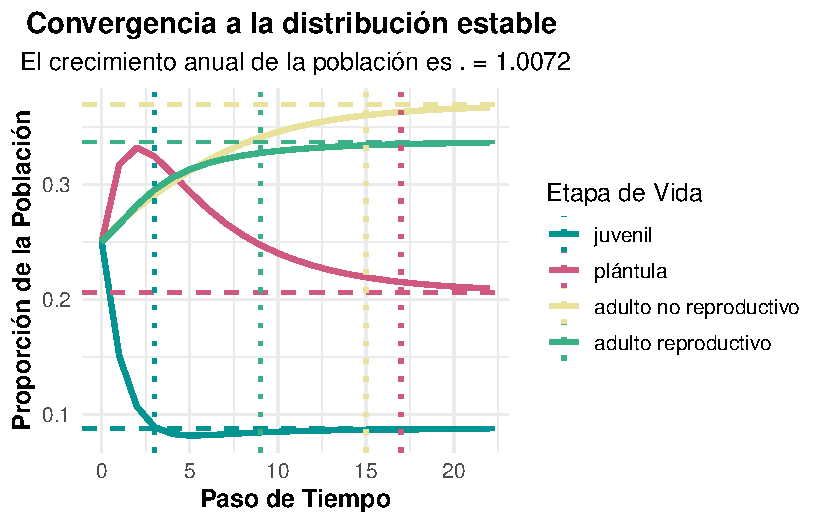
\includegraphics{110-Propriedades_files/figure-pdf/indice16-1.pdf}

Revisión:

RLT 2025\_06\_02

RLT 2025-11-22

\phantomsection\label{refs}
\begin{CSLReferences}{1}{0}
\bibitem[\citeproctext]{ref-caswell2001matrix}
Caswell H. 2001. \emph{Matrix {P}opulation {M}odels: Construction,
analysis, and interpretation}. Sunderland, Massachusetts, USA: Sinauer
Associates.

\bibitem[\citeproctext]{ref-crone2011plant}
Crone EE, Menges ES, Ellis MM, Bell T, Bierzychudek P, Ehrlén J, Kaye
TN, Knight TM, Lesica P, Morris WF, others. 2011. How do plant
ecologists use matrix population models? \emph{Ecology Letters} 14:1--8.

\bibitem[\citeproctext]{ref-jiang2020life}
Jiang S, Jaggi H, Zuo W, Oli MK, Gaillard J-M, Tuljapurkar S. 2020.
Life-history dynamics: Damping time, demographic dispersion and
generation time. \emph{bioRxiv}:2020--12.

\bibitem[\citeproctext]{ref-mangalam2022ergodic}
Mangalam M, Kelty-Stephen DG. 2022. Ergodic descriptors of non-ergodic
stochastic processes. \emph{Journal of the Royal Society Interface}
19:20220095.

\bibitem[\citeproctext]{ref-stott2011framework}
Stott I, Townley S, Hodgson DJ. 2011. A framework for studying transient
dynamics of population projection matrix models. \emph{Ecology Letters}
14:959--970.

\bibitem[\citeproctext]{ref-tremblay2015stable}
Tremblay R, Raventos J, Ackerman J. 2015. When stable-stage equilibrium
is unlikely: Integrating transient population dynamics improves
asymptotic methods. \emph{Annals of Botany} 116:381--390. DOI:
\href{https://doi.org/10.1093/aob/mcv031}{10.1093/aob/mcv031}.

\bibitem[\citeproctext]{ref-williams2011distance}
Williams JL, Ellis MM, Bricker MC, Brodie JF, Parsons EW. 2011. Distance
to stable stage distribution in plant populations and implications for
near-term population projections. \emph{Journal of Ecology}
99:1171--1178.

\end{CSLReferences}


\backmatter


\end{document}
